\documentclass[12,twoside]{TFG-GM}
%\usepackage[active]{srcltx}
\usepackage{amsthm,amsmath,amssymb,amsfonts,amscd}
\usepackage{graphicx}
\usepackage{enumerate}
\usepackage[all]{xy}
\usepackage{booktabs}
\usepackage{cite}
\usepackage{url}
%\usepackage[usenames]{xcolor}
%\usepackage{fancyhdr}

%%%%%Author packages if necessary

\usepackage{algorithm}
\usepackage[noend]{algpseudocode}

% Theorem Environments: add extra ones at the end if you need it.

\newtheorem*{theoremA}{Theorem A}
\newtheorem{theorem}{Theorem}[section]

\newtheorem{proposition}[theorem]{Proposition}
\newtheorem{lemma}[theorem]{Lemma}
\newtheorem{assumption}[theorem]{Assumption}
\newtheorem{corollary}[theorem]{Corollary}
\newtheorem{conjecture}[theorem]{Conjecture}

\theoremstyle{definition}
\newtheorem{definition}[theorem]{Definition}
\newtheorem{example}[theorem]{Example}

\theoremstyle{remark}
\newtheorem{remark}[theorem]{Remark}
\newtheorem*{remarknonumber}{Remark}
\newtheorem{observation}[theorem]{Observation}




%%%%%%%%%%%%%%%%%%
% macros/abbreviations: Include here your own.
%%%%%%%%%%%%%%%%%%

\newcommand{\N}{\ensuremath{\mathbb{N}}}
\newcommand*\mean[1]{\bar{#1}}
\newcommand*\diff[1]{\bar{#1}}

% Body of document

\titol{A Learning Approach\\[3mm] To The FOM Problem}
\titolcurt{A learning approach to the FOM problem}
\authorStudent{Eudald Romo Grau}
\supervisors{Alberto Rodriguez Garcia and Maria Alberich Carrami\~nana}
\monthYear{April, 2017}

%\msc[2010]{Primary  	55M25, 57P10, Secondary 55P15, 57R19, 57N15.}

\paraulesclau{Manipulation, Online Control, MPC, FOM, Underactuation, Hybridness}
\agraiments{
Thanks to Alberto Rodriguez for tutoring my research, for providing me with the required tools and financial support to undertake this project and for hosting me in his laboratory; to Maria Alberich for supervising and tutoring this thesis; to Fran\textbf{c}ois Hogan for sharing his ideas on family of modes trajectory control and for introducing me to his previous work, to Maria Bauza for sharing with me her insights in machine learning techniques; to Nikhil Chavan-Daffle for sharing with me his insights in complementarity constraint problems; to all the members of the MCube Lab for sharing their thoughts on my research, to Centre de Formacio Interdisciplinaria Superior for offering me the possibility and the financial support to take part in this project, to Massachusetts Institute of Technology for providing the required facilities required to develop this project and to Generalitat de Catalunya for their financial support.}


\abstracteng{The family of modes (FOM) approach to solving model predictive control (MPC) problems is a novel heuristic technique developed at MIT to solve the time complexity of traditional MPC solving techniques. This study addresses some of the issues associated with the previous formulations of this technique by increasing the sequential robustness of the FOM and providing methodologies to choose the parameters required for the heuristic. A general simulation interface is developed together with techniques to score and compare the obtained trajectories. Then an statistics and machine learning based methodology to tune the parameters is proposed and the results are compared with the original ones. Finally, experimental procedures are developed to validate the results.}

%%%%%%%%%
\begin{document}

\maketitle

                                                                      
\section{Goal of this study}
\label{briefgoal}
Hogan \cite{fom} recently provided an heuristic technique called family of modes (FOM) to solve model predictive control (MPC) problems under hybrid constraints and underactuation. The goal of this study, that will be revisited and expanded in section \ref{sec:goal_revisited}, is to further develop this new method and to expand its usage in the robotics manipulation community.

In order to do that, we reinforce the method by fixing some of it's weaknesses -as it's sequential properties-, we provide comparison tools to test the method against traditional hybrid MPC solving techniques -as mixed integer quadratic programming (MIQP)-, and to provide simple and systematic techniques to optimize a general MPC problem.

To proof the scalability of this method we increase the complexity of the systems beyond the problem used in Hogan's work -tracking straight lines with of a single point pusher and a square slider.

Some simple control policies as proportional–integral–derivative (PID) controllers are able to control systems that scape the model they were designed for. Inspired by this fact, we check the robustness of the FOM method by using it in models that are different from those it is designed for.

In section (TODO: add conclusion/discussion section) we discuss the new lines of research we plan on exploring before presenting this study to 2017's International Symposium on Robotics Research (ISRR). We hope that the results from our studies will increase the performance and simplify the implementation of FOM and will bring it closer to the robotics manipulation research community by both providing systematic set-up tools and showing it's robustness and scalability.

In the following sections we introduce the concepts of manipulation problems under hybridness required to explain the FOM method and show its motivation.

\section{Planar Pushing}
\label{sec:intro}

As Mason explained in his talk during his CITRIS People and Robots Seminar Series talk \cite{mason_talk}, robotics manipulation research has been traditionally based on a pick and place methodology that consisted in solving two fundamental problems:
\begin{enumerate}
\item{ \textbf{Determine a stable grasping configuration:}} A stable grasping configuration was generally obtained by finding a set of points that completely constrained the picked object position and orientation with respect to the gripper.
\item{ \textbf{Solving a collision-free trajectory planning problem:}} Once the object was grasped it was rigidly attached to the robot gripper and the trajectory planning problem was completely determined at every point.
\end{enumerate}

This methodology was constantly improved as the manipulation community considered broader and more complex problems, as Rodriguez' and Mason's study \cite{caging}, that generalized the concept of stable grasp to caging -a partial immobilization of the grasped object that allows it to move in a bounded space. Other modifications added further constraints to the problem, as the concept of compliant grasping manipulation \cite{compliant_control}, where the object motion of the object is constrained by the task and the constraint is enforced without exerting heavy force loads on the object. An example of compliant manipulation the process of activating a lever. The lever only has one degree of freedom and can easily be broken by small planning uncertainties if a powerful robotic arm is used and the trajectory is controlled uniquely with the robot position without considering the applied forces. It should be noted that all these variations were applied to the same pick and place grasping problem. Some of the main motivations that made stable grasping so popular are:
\begin{itemize}
\item {\textbf{Easy to track:}} The obtained solutions are constrained by the contact points and the gripper pose so, even if the object could move inside the gripper (as in cagings) the object position could be deterministically bounded during all the trajectory.
\item {\textbf{Robustness:}} Most grasping point predictions are robust to small sensor noise and applying enough grasping force allows ignoring uncertainties in the grasped object friction coefficients.
\item {\textbf{Simplicity:}} As explained, the manipulation problem could be formulated simply by a grasping point identification and a path planning problem.
\end{itemize}

At least as far as on 1980's, some drift towards the study of the mechanics of planar pushing started to appear with studies as Mason's \cite{pushing4}.
The main motivations for this drift were to handle problems that were not tractable with grasping or to better understand the grasping mechanics. A non-exhaustive list of the motivations of planar pushing could be:
\begin{itemize}
\item {\textbf{You don't need to lift:}} Lifting heavy objects using a traditional robotic arm can put heavy torque strain on the arm in certain arm configurations and the strain can break or topple the arm. If most or all of the planned trajectory can be done through pushing, the required force is usually reduced and when the maximum force is achieved safety mechanisms can be implemented so that the arm doesn't break.
\item {\textbf{Sometimes you need to push to grasp:}} From the observation of human object handling, it can be seen that sometimes we prefer or need a previous pushing manipulation before grasping an object. As can be observed in Figure \ref{fig:book}, constrained spaces like a shelf may force us to previously push a book against one of the self walls to pull it outside so that we can grasp it.
\item{\textbf{It Can Represent In-Hand Re-grasping:}} Humans constantly show the ability and need to modify a grasping configuration without letting the object out of the grasp. When we write with a pen or drink from a bottle, we are constantly adapting our initial grasp without letting the object go to achieve more comfortable configurations. Some studies as Chavan's \cite{nik1} \cite{nik2} have formulated this in-hand re-grasping as a planar pushing problem by considering either one moving finger or an external surface as the pusher and the contact between the fixed fingers and the object is described as planar sliding.
\item{\textbf{Weaker Quasistatic Assumptions:}} As will be further explained in section \ref{subsec:quasistatic}, in order to use quasistatic grasping analysis (commonly done in the manipulation community) a stronger set of assumptions has to be taken than to use quasistatic pushing.
\end{itemize}

\begin{figure}[htb!]
\begin{center}
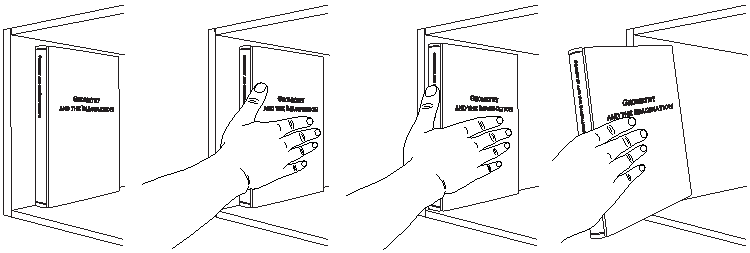
\includegraphics[width=16cm]{ManipulationBook.pdf}
\end{center}
\caption[test caption]{\label{fig:book} \small{Figure from \protect\cite{fom} that shows a human-like book grasping procedure.}}
\end{figure}

The mechanics of planar pushing are complex and contain some inherent qualities as underactuation and hybridness that need to be addressed in order to solve planning, simulating or control problems. In the following sections we are going to introduce the basic assumptions taken and models used in planar pushing, together with the difficulties that arise from them.

\subsection{Coulomb Friction}
\label{subsec:coulomb}
One of the usual assumptions in the robotics community is considering dry Coulomb contact forces. This model separates friction into two possible states (static and dynamic or kinetic friction) and the set of rules which describe it are a combination the work of Amontons \cite{amontons} and Coulomb \cite{coulomb_law}:
\begin{itemize}
\item{Amontons's first law:} The force of friction is directly proportional to the applied load.
\item{Amontons's second law:} The force of friction is independent of the apparent area of contact.
\item{Coulomb's law:} Kinetic friction is independent of the sliding velocity.
\end{itemize}

This laws are usually condensed by defining the static ($\mu_s$) and kinetic ($\mu_k$) coefficients and considering the normal ($f_n$) and tangential ($f_t$) components of the contact force:

\begin{theorem} \textbf{Coulomb's Law:}
\[
  f_t\begin{cases}
               < \mu_s \cdot f_n   \text{ (for static contact)}\\
               = \mu_k \cdot f_n   \text{ (for kinetic contact)}\\
            \end{cases}
\]
Where $f_t$ is determined in the first situation by force balancing.
\end{theorem}

\begin{remark}
Through the rest of this thesis we use the common assumption taken in robotics manipulation of assuming a single coefficient of friction. Thus the previous theorem is simplified to $f_t \leq \mu \cdot f_n$
\end{remark}

Mason cites prior statements by Da Vinci (from Truesdell's notes \cite{da_vinci}) and experimental verification by Truesdell and Guillmor \cite{gillmor} and I would like to add the work of Euler \cite{euler}, who first distinguished between static and kinetic friction.

\subsection{Contact Slider-Support Surface}
\label{subsec:planar_sliding}
In planar pushing, there are two different contacts to be considered: the contact between the object (slider) and the support surface and the contact between pusher and slider. In this section we are going to introduce the main theoretical results about the first one. We will start with Mason's study of the relation between friction force and both motion and instantaneous center of rotation (which will be used again in section \ref{subsec:quasistatic}) and we will end with Goyal's Limit Surface, that will provide a geometric interpretation to this relation.

The contact between the slider and the support surface is inherently complex. If the slider is supported by more than three contact points the distribution of support normal forces is indeterminate and, if Coulomb contact is assumed, this indetermination is propagated to the friction forces. The results in this section are based on the previous assumption that the pressure distribution is known (for our study we will consider a homogeneous distribution).

Assuming a known pressure distribution and considering \textbf{r} the position vector of a point of the slider, \textbf{v(r)} it's velocity vector, and p(\textbf{r}) the pressure at that point, then the total force and moment due to friction can be expressed as:
\begin{definition} \textbf{Total force due to friction:} 
\begin{equation}
\textbf{f}_f = - \mu \int_A \dfrac{\textbf{v(r)}}{|\textbf{v(r)}|} p(\textbf{r}) dA
\end{equation}
\end{definition}
\begin{definition} \textbf{Total moment due to friction:}

\begin{equation}
n_f = - \mu \int_A \textbf{r} \times \dfrac{\textbf{v(r)}}{|\textbf{v(r)}|} p(\textbf{r}) dA
\end{equation}
\end{definition}

If the slider trajectory is assumed to be a rotation over a instantaneous center $\textbf{r}_{IC}$, the velocity can be expressed as $\textbf{v(r)} = \omega \times (\textbf{r} - \textbf{r}_{IC}) = $ and the previous results can be rewritten as:
\begin{definition} \textbf{Total force due to friction:} 
\begin{equation}
\textbf{f}_f = - \mu \, sgn(\dot{\theta}) \, \hat{\textbf{k}} \times \int_A \dfrac{\textbf{r} - \textbf{r}_{IC}}{|\textbf{r} - \textbf{r}_{IC}|} p(\textbf{r}) dA
\end{equation}
\end{definition}
\begin{definition} \label{def:} \textbf{Total moment due to friction:}
\begin{equation} \label{eq:momentum_cor}
n_f = - \mu  \, sign(\dot{\theta}) \int_A \textbf{r} \cdot \dfrac{\textbf{r} - \textbf{r}_{IC}}{|\textbf{r} - \textbf{r}_{IC}|} p(\textbf{r}) dA
\end{equation}
\end{definition}

\begin{remark} 
These equations are well defined when the magnitude of $\textbf{r}_{IC}$ tends to infinity and they correspond to pure translations perpendicular to it.
\end{remark}

These equations provide a relation force-motion for known continuous pressure distributions but if non-zero support force is allowed at discrete points, they become undefined for rotations about each of them. In fact, the relation between motion and frictional force cannot generally be described as an analytical function. Goyal et al. \cite{planar_sliding1}\cite{planar_sliding2} applied concepts of classical plastic theory to describe planar sliding, deriving the concepts of limit surfaces for dry contact manipulation, that describe a mapping between motion and force.

Goyal's work can be generalised to friction models which are more general but, for clarity, the main concepts will be introduced with the special case of isotropic Coulomb friction (as was presented in their original paper).

Consider a rigid body sliding over a surface with a known or pressure distribution p(\textbf{r}) at every contact point and assume that each point of contact follows isotropic Coulomb friction law. Let \textbf{f(r)} be the differential frictional force applied by each slider particle to the surface. Coulomb law allows us to obtain two important properties:
\begin{enumerate}
\item {\textbf{Limit Curve:}} The set of possible point differential friction forces is contained inside a circle of radius $\mu  p(\textbf{r})$ centred at the origin of the force space. We will call this circle the limit curve (LC) of each contact point.
\item {\textbf{Maximum Power Inequality. }} The following relation is held at every contact point:
$$ \forall \textbf{f(r)}^* \in LC: \,\, (\textbf{f(r)} - \textbf{f(r)}^*)\cdot \textbf{v(r)} \geq 0 $$
Where \textbf{v(r)} is the point velocity at each contact point and $\textbf{f(r)}^*$ is an arbitrary force that can take any possible value inside the LC.
\end{enumerate}

The maximum-power inequality and limit curve are concepts introduced from classical plastic theory that can be interpreted as follows: when slip occurs \textbf{v(r)} is non-zero and, for the case of a circular LC, the maximum power inequality restricts \textbf{f(r)} to have the same direction as \textbf{v(r)} and lie on the LC boundary. That is, the frictional load is on the limit curve and the motion vector is normal to the limit curve at \textbf{f(r)}. When the point velocity is zero, the frictional load is undetermined.

\begin{figure}[htb!]
\begin{center}
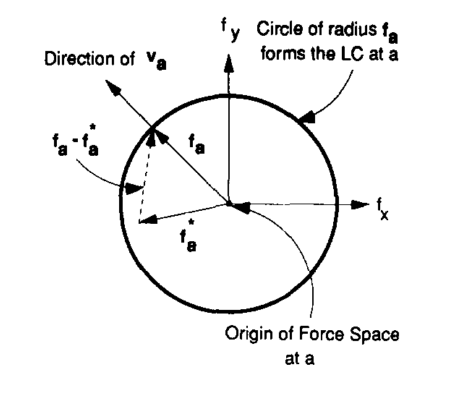
\includegraphics[width=10cm]{isotropic_lc.png}
\end{center}
\caption[test caption]{\label{fig:iso_lc} \small{Figure from \protect\cite{planar_sliding1} that shows a limit curve for isotropic Coulomb contact at a certain position \textbf{$r_a$}. A unique set of \textbf{$v_a$} and \textbf{$f_a$} is determined when the point is slipping and it corresponds to the points in the circumference. When the force lies inside the circle, the point does not move and the frictional force is not determined.}}
\end{figure}

Goyal's study further uses classical results of plastic theory to generalize this concept to general closed LC that are convex (to allow the maximum power inequality to be held at every contact point) and that enclose the origin of the force space (to allow positive energy dissipation). The motion-force relationship properties obtained in this general LC study are summarized in Figure \ref{fig:general_lc} and explained here:

\begin{enumerate}
\item If \textbf{f(r)} is in the interior the LC, then \textbf{v(r)} is zero.
\item If \textbf{f(r)} is on a LC boundary point with a well-defined normal, then \textbf{v(r)} is perpendicular to the LC.
\item If \textbf{f(r)} is on a LC vertex, the direction of \textbf{v(r)} is not determined.
\item For all \textbf{f(r)} in a same flat region of the LC, a common \textbf{v(r)} value is associated, perpendicular to the LC, so the direction of \textbf{f(r)} is not determined given \textbf{v(r)}
\end{enumerate}

\begin{figure}[htb!]
\begin{center}
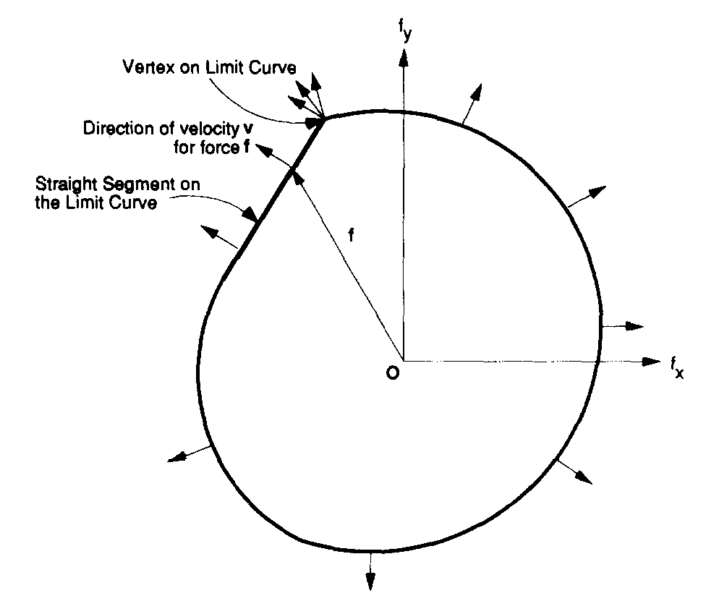
\includegraphics[width=10cm]{general_lc.png}
\end{center}
\caption[test caption]{\label{fig:general_lc} \small{Figure from \protect\cite{planar_sliding1} that shows a general limit curve at a certain contact point. The four possible motion-force relations are represented on it.}}
\end{figure}

If we consider \textbf{p} the total frictional load wrench
$$ \textbf{p} =
  \begin{pmatrix}
    f_x \\
    f_y \\
    n_{0z}
  \end{pmatrix} = \sum_r \begin{pmatrix}
    f_x(\textbf{r}) \\
    f_y(\textbf{r})\\
    \textbf{r} \times \textbf{f(r)}
  \end{pmatrix}   $$
and \textbf{q} the velocity twist
$$ \textbf{q} =
  \begin{pmatrix}
  v_{0x} \\
  v_{0y} \\
  \omega_z
  \end{pmatrix}
$$
then Goyal's study generalizes the concept of single point Limit Curves for force-motion relationship to Limit Surfaces(LS) that relate total wrench and twist for the slider:
\begin{theorem} \textbf{Limit Surface:}


\begin{enumerate}
\item The set of possible load wrenches \textbf{p} is contained inside a LS.
\item The following relation is held at every contact point:
\begin{equation}
 \forall \textbf{p}^* \in LS: \,\, (\textbf{p} - \textbf{p}^*)\cdot \textbf{q} \geq 0 
\end{equation}
\end{enumerate}
\end{theorem}

Certain properties are derived for the LS and we are going to list here without proof the ones that apply to our study:
\begin{itemize}
\item With isotropic friction, flat regions appear on the limit surface if
and only if it has points of finite support (infinite stress).
\item With isotropic friction, vertices appear on the limit surface if and
only if all support points lie on one straight line segment.
\end{itemize}

When smooth enough, the limit surface allows to compute the frictional wrench from a non-zero motion twist, but it should be noted that the reciprocal relation can never be obtained (except for the trivial case where the wrench is inside the surface and the twist is zero), but the twist direction can be obtained successfully. As will be discussed in chapter \ref{sec:formulation}, combining the constraints obtained from this relation with other constraints applied on the Pusher-Slider contact, the motion equations for the pusher slider can be derived.

\subsection{Contact Pusher-Slider. Friction Cone And Hybridness}
\label{subsec:frictioncone}
The contact between the pusher fingers and the slider sides could be described as in the previous section (by considering the finger a slider and the slider side a support surface) but the nature of the problem allows some simplifications. The fingers we consider never rotate with respect to the slider side, so all the motion is pure translation. Furthermore, we only consider planar pushing (we do not consider operations as tilting the slider), so we are only interested in moving the pusher along one dimension of the slider face (for most purposes we consider the slider to be flat).

A common and useful geometric interpretation of Coulomb's law called the friction cone (according to Mason first constructed by Moseley \cite{moseley}) is widely used in the robotics community for one dimensional single point contacts. Given a point on a surface interacting with it with total contact force \textbf{f}, we decompose it into its normal $f_n$ and tangential $f_t$ components with respect to the contact surface. Coulomb friction compact formulation states that $f_t \leq \mu f_n$, where $\mu$ is the proportionality factor usually called friction coefficient, where the equality holds on dynamic friction. Letting $\alpha$ be the angle between \textbf{f} and $f_n$ (or, alternatively, the normal of the surface on the point of contact), Coulomb's law is equivalent to: %TODO: Change slide Up/Down to right/left

\begin{theorem} \label{th:friction_cone} \textbf{The set of feasible forces in dry Coulomb contact must satisfy:}
$$\alpha := tan^{-1} \frac{f_t}{f_n} \leq \mu$$
\end{theorem}

So, the set of feasible contact forces lies inside a closed cone with aperture $2\mu$.

\begin{figure}[htb!]
\begin{center}
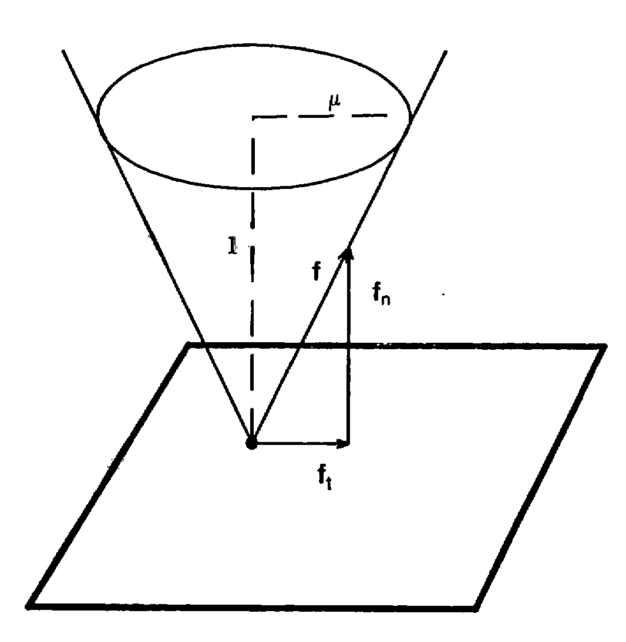
\includegraphics[width=10cm]{friction_cone.png}
\end{center}
\caption[test caption]{\label{fig:book} \small{Figure from \protect\cite{pushing4} that shows the friction cone, the geometric interpretation of Coulomb's Law. The set of all vectors following.}}
\end{figure}

Consider a single point finger pushing a planar slider. There are three possible contact states: The finger can stick to the slider (Sticking State), the slider can slide with a slip to the left relative to the finger (Sliding Left State) or it can slide with slip to the right (Sliding Right State). This section shows that in each state the pusher can apply a different range of forces to the slider. Each of this different range of forces will translate into different ranges of friction reactive wrench, that will ultimately lead to different slider twist ranges.

This multiple system state phenomenon (inherent in Coulomb Contact) is commonly referred as hybridness. Hybridness appears in many manipulation situations different than sticking/sliding ones. For example a gripper can throw the object in the air to re-grasp it, change the number of fingers contacting the object, change the pusher-slider contact side while pushing a slider of irregular shape, etc. It also appears in other robotic fields as locomotion, where there are always at least two differentiated states (aerial state and ground state) with clearly different dynamics. 

In the following chapter, we are going to discuss the hybridness phenomenon in more detail by covering why is it important to take into account, the problems that arise when considering hybridness in planning and control problems and different methods to solve them in each field, that will ultimately lead to the introduction to the FOM method.

\section{Hybridness in Manipulation Problems}

Through all this section, we will compare the role of hybridness in different aspects of manipulation problems. The principal fields we will distinguish are  simulation, trajectory planning and trajectory control. Each of these fields take a different role when studying a general manipulation problem, that we can generally defined as follows:
\begin{definition} \textbf{Manipulation Problem:}\\

Given a system conformed by a set of points in a metric space M and a parametrization $c(\textbf{x})$ (for \textbf{x} in a certain configuration space C) that uniquely describes the position of all the points of interest in the metric space, a manipulation problem consists in changing a certain initial configuration $\textbf{x}_0$ into a final configuration \textbf{$\textbf{x}_f$} following appropriate constraints.
\end{definition}

Simulation problems consist on accurately reproducing the real physics of a manipulation problem to safely and quickly study its properties. A key property of most simulation problems is that, at every instant of time, we know the configuration of the system until the current time step and the only variables we need to compute are the ones that define the configuration in the next step.

Planning problems consist on finding a trajectory in the configuration state to go from state $\textbf{x}_0$ to $\textbf{x}_f$. Most simple planning problems have a state variable that defines the configuration of the object we need to manipulate and a actuator state variable that describes the configuration of the gripper or other tool used to move the object. As opposed to simulation problems, planning problems don't have full information about the state of the object and actuator state variables for each step of the trajectory, and they are usually variables of the problem. Because of this difference, the equations that describe the evolution of the same actuator-object system can have different properties in planning or simulation problems. As an example, the motion equations we derive in section \ref{subsec:motion_equations} are generally non-linear (they are linear with respect to the object state variables but not with respect to the actuator state variables), but they can be expressed as linear equations on the actuator state variables for the first step of the problem, where we know the initial state of the object.

Traditional control designs as PID controllers can successfully control a system by solving only local manipulation problem, in a similar way as simulation. PID only use the notion of the current and past differences between the configuration of the object \textbf{x} and it's objective value $\textbf{x}^*$ to devise a control response to stabilize the realized trajectory around the objective one. Such control cannot be used for pushing because of a phenomenon called underactuation.

TODO: Add the concept of WHY Should we care about hybridness here

\label{sec:hybridness}
\subsection{Underactuation. Trajectory Optimization}

A control problem with first order motion constraints $\dot{\textbf{x}}$ = f({\textbf{x}, \textbf{u}}) for some control input \textbf{u} is underactuated when f is non-exhaustive in the configuration velocities space. In most problems, $\dot{\textbf{x}}$ is the result of converting a second order Newtonian equation $\ddot{\textbf{x}} = m\sum F$ to a system of first order ordinary differential equations (ODEs) and underactuation is usually caused by the controller being able to transmit only a limited set of forces and moments to the object.
 
In stable grasping, the system is fully activated (see remark \ref{rem:underactuation}) at all times. On the other hand, for a single simple point finger pushing the system is highly underactuated, as the normal force the pusher applies to the slider is non-negative (there cannot be no pulling forces) and the overall contact force lies in the friction cone. As such, the controller must reason only among the forces that can physically be realized at every instant.

In a certain way, it can be considered that underactuation distorts the usual metric of the system. The example in Figure \ref{fig:underactuation} shows a tracking problem where a single point pusher needs to move a square slider to a configuration situated just behind the current pusher location. Any local pushing control action will bring the system away from the objective configuration if we use a tradition 2D Euclidean metric. If the controller takes into account a certain notion of path and future and tries to minimize the overall distance through the considered control trajectory, it can obtain a solution like the one we show.

\begin{remark} \label{rem:underactuation}
Stable grasping has some some sources of underactuation, but they are linked with the situations were the stable grasp property cannot be held. For example, if an object is too heavy to be lifted or to be kept in a grasp without slipping. These are examples of underactuation, as the gripper cannot transmit enough force to the object, but they are also examples where stable grasping is not possible.
\end{remark}


\begin{figure}[htb!]
\begin{center}
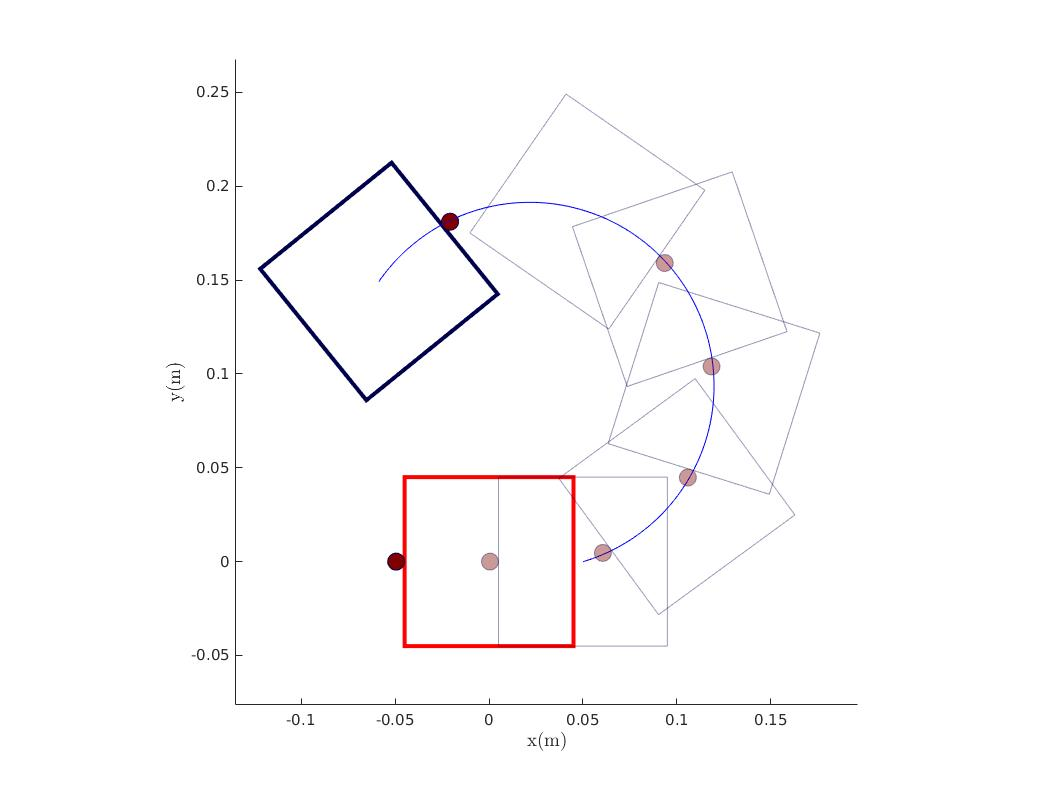
\includegraphics[width=15cm]{underactuation.jpg}
\end{center}
\caption[test caption]{\label{fig:underactuation} \small{Control trajectory obtained when trying to bring the slider to a configuration behind the current position of the pusher. The red slider describes the objective configuration, the blue line describes the trajectory of the slider center of mass during the control trajectory and the blue sliders represent some of the configurations of the system during the tracking trajectory. The position of the slider when we stopped the simulation is highlighted with thicker and more opaque lines.}}
\end{figure}

A common method to consider future paths in control problems is to solve simplified planning problems at high frequency. The planning problems can usually be expressed as trajectory optimization problems, where the values of the state and control variables are chosen to minimize a cost function along the trajectory, while fulfilling the required motion constraints that represent the kinematics of the real world problem. These optimization problems are usually linearized around the nominal trajectory computed by a planning problem beforehand. This linearization reduces the computational cost of the control problem while ensuring that, in a certain region of attraction, the controlled trajectory converges to the nominal one. It's also common to only consider the control path until a certain finite time horizon (as opposed to planning problems, that usually consider the trajectory until reaching a certain goal).

Once stated the need to consider trajectories in pushing control problems we will now justify the need to consider hybridness in the control problems. This justification is threefold:

\begin{itemize}
\item {\textbf{Optimality:}}
\item {\textbf{Robustness:}}
\item {\textbf{Convergence:}}
\end{itemize}

In the next sections we will introduce formulation techniques to add the hybridness concept into manipulation problems. In particular, we will discuss the limitations of some of the formulations to solve control problems at enough frequency. This will ultimately lead to Hogan's FOM formulation as an approximate method to solve the finite horizon trajectory optimization problem.

\subsection{Complementarity Problems}
\label{subsec:comp_prob}
Given a variable \textbf{z} and a function on it \textbf{g(z)}, a general complementarity problem consists on finding a value for \textbf{z} that satisfies:
$$ \textbf{z} \geq 0 \,\,\,\,\,\,\,\,\,\, \textbf{g(z)} \geq 0 \,\,\,\,\,\,\,\,\,\, \textbf{g(z)} \cdot \textbf{z} = 0$$

This formulation derives from traditional linear programming techniques to encode two mutually exclusive constraints on \textbf{z} ($\textbf{z} \geq 0$ and $\textbf{g(z)} \geq 0$). The linear complementarity problem (LCP) \cite{compconst} assumes a linear g function and takes the following form:
$$\boldsymbol{\omega} = \textbf{R} \textbf{z} + \textbf{u} $$
$$	\boldsymbol{\omega} \geq 0 \,\,\,\,\,\,\,\,\,\, \textbf{z} \geq 0 \,\,\,\,\,\,\,\,\,\, \boldsymbol{\omega}^{T} \cdot \textbf{z} = 0$$
It was first introduced to predict instantaneous acceleration of rigid bodies in 1996 by Pang and Trinkle \cite{lcpi} and Anitescu and Potra \cite{lcc1}, that guaranteed a solution for this formulation on multi-rigid-body Coulomb friction contact and impact problems. This provided a systematic way to formulate hybrid constraints for simulation purposes. Soon after the instantaneous formulation introduction, Steward and Trinkle \cite{lcpd} proposed a time-stepping formulation in the space of impulses and velocities which increased the stability performance of LCP based forward simulation techniques.

\begin{remark}
It should be noted that the LCP formulation of the multi-rigid-body Coulomb friction problems used a polyhedral approximation to the friction cone.
\end{remark}

There are fast algorithms to solve LCP problems that allow the manipulation community to use them in simulation, as in Steward and Trinkle's study \cite{lcpd}, or other instantaneous-nature problems as the studies of Fazeli et al. to identify friction parameters from observed object motions \cite{fazeli2015identifiability} \cite{fazeli2016parameter}.
\begin{figure}[htb!]
\begin{center}
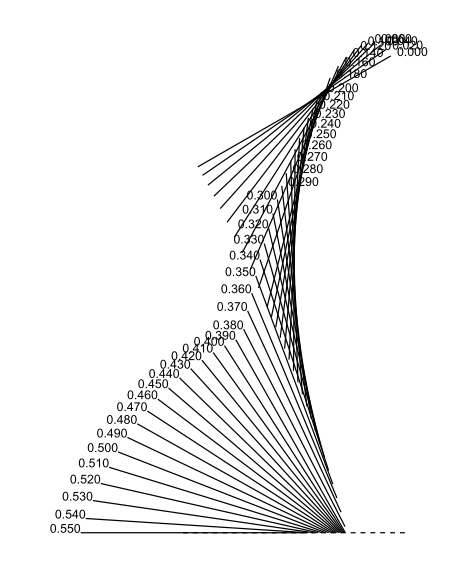
\includegraphics[width=10cm]{lcp.png}
\end{center}
\caption[test caption]{\label{fig:lcp} \small{Figure from \protect\cite{lcpd} with the simulation results obtained when emulating a falling and spinning rod. The simulation step was h = 0.0025 and the simulation time at each time instant is shown in seconds on one of the bar ends.}}
\end{figure}

In instantaneous Coulomb contact problems the contact dynamics can be expressed in linear discrete form through Steward and Trinkle's formulation,

TODO: talk with nikhil more about it but a key property of their formulation is that they know the value of the velocity and forces prior to contact.  but this cannot be applied to contact-driven trajectories. The problem becomes nonlinear (NCP) and an instance of the NCP has to be used to compute the contact state at each point in the discretization of the trajectory.

LCP can not be used as is to solve problems which also contain non-complementarity subject variables that must hold linear constraints. Luckily, these problems, called mixed LCP (MLCP) can also be solved with a generalization of Lemke's algorithm, the key idea used to provide the LCP solution. Nikhil's work on extrinsic dexterity \cite{nik1} is an example of MLCP usage in planning. 

\subsection{MPC and MIQP}
\label{subsec:MPC}

MLCP is usually too slow to be used in trajectory optimization based control problems. Complementarity constraints are generally non-convex, which makes it difficult to use them in other algorithms than LCP or MLCP problems. To tackle the computing cost of complementarity constraints, model predictive control(MPC) can be used. Given an initial state $\diff{\textbf{x}}_0$, an MPC problem consists in defining a discrete set of N positions $(\diff{\textbf{x}}_1, ..., \diff{\textbf{x}}_N)$ and control inputs $(\diff{\textbf{u}}_0, ..., \diff{\textbf{u}}_{N-1})$ to define a trajectory a trajectory. $\diff{\textbf{x}}_i = \diff{\textbf{x}}(t_j)$, where $t_j = t_0 + h j$ for a certain time step h. Similarly, $\diff{\textbf{u}}_i$ stands for the control input necessary to transition from $\diff{\textbf{x}}_i$ to $\diff{\textbf{x}}_{i+1}$. Given this notation, MPC optimizes the values of all $\diff{\textbf{x}}_i$ and $\diff{\textbf{u}}_i$ with respect to a certain cost function:
\begin{equation} \label{eq:cost_function}
J(\diff{\textbf{x}}_0, ..., \diff{\textbf{x}}_N, \diff{\textbf{u}}_0, ..., \diff{\textbf{u}}_{N-1}) = \diff{\textbf{x}}_N^T \textbf{Q}_N \diff{\textbf{x}}_N^{} + \sum\limits_{i = 0}^{N-1} \left( \diff{\textbf{x}}_i^T \textbf{Q} \diff{\textbf{x}}_i^{} + \diff{\textbf{u}}_{i}^T \textbf{R} \diff{\textbf{u}}_{i}^{} \right)
\end{equation}

Where terms \textbf{Q}, $\textbf{Q}_N$, and \textbf{R} are weights matrices that penalize the error state, final error state, and control input, respectively. MPC problems consider the hybrid state to be constant during state state transitions. Under this assumption, a hybrid mode can be defined:

\begin{definition} \label{def:mode} A \textbf{hybrid mode} is a ordered set of hybrid states.

In MPC, an N-length mode completely fixes the hybrid states the system is in along the finite horizon considered trajectory.
\end{definition}


\begin{remark}
We use the $\diff{(.)}$ notation because, as will be explained in sections \ref{subsec:motion_equations} and \ref{subsec:mpc_formulation}, we will use the perturbation of the state and control variables with respect to a nominal trajectory and control inputs as the MPC variables.
\end{remark}
\begin{remark}
MPC problems are based in the linear quadratic regulators (LQR) controllers. These controllers are used for unconstrained non-hybrid problems described by the motion equation $\dot{\textbf{x}} = \textbf{A} \cdot \textbf{x} + \textbf{B} \cdot \textbf{u}$ and use the same cost functions as MPC. LQR are able to give an analytical control law to minimize the cost function provided for infinite horizon problems. Their term $\textbf{Q}_f$ can be set-up to account for the integral of the cost function from the last point considered until reaching the destination (if the trajectory is finite) or until infinite. If the $\textbf{Q}_f$ term is chosen to follow the Riccati equation $\textbf{Q}_f = \textbf{A}^T \cdot \textbf{Q}_f \cdot \textbf{A} - \textbf{A}^T\cdot \textbf{Q}_f\cdot \textbf{B}\cdot(\textbf{B}^T\cdot \textbf{Q}_f \cdot\textbf{B} + \textbf{R})^{-1}\cdot \textbf{B}^T \cdot\textbf{Q}_f \textbf{A} + \textbf{Q}$, the finite horizon LQR controllers will behave as the infinite horizon ones. In MPC problems there's no closed expression for this term but there are certain techniques to choose a good value to maximize the final region of attraction as the one exposed in Ya-Feng's et al. study \cite{riccati}, but it is generally based on the LQR technique of solving the Riccati equation . In our model we use a simplification of Ya-Feng's approach which simply computes the solution of the Riccati equation presented above using the motion equation of the last MPC step, that can be expressed as $\dot{\textbf{x}} = \textbf{A}_N \cdot \textbf{x} + \textbf{B}_N \cdot \textbf{u}$.
\end{remark}

If we consider a manipulation problem with convex dynamics, constraints, and cost function, the overall optimization problem is convex if a hybrid mode that describes the finite horizon is provided. Thus, the global problem consists in selecting the optimal solution from the finite set of optimal solutions for each of the fixed-mode sub-problems.

The number of possible modes of length N is $h^N$, where h is the number of possible hybrid states. This exponential growth generally makes a naive exploration of all the possible sub-problems too computationally expensive. In order to reduce the algorithmic strain, a mixed integer programming (MIP) strategy is usually adopted. This will be further explained in chapter \ref{sec:formulation}, but the main idea is that the state space is expanded by adding h binary variables per MPC step that define whether the step i of the MPC is in a hybrid state s. The commercial optimizers provide tools to express state the state related constraints with respect to each of this binary variables so that they only apply when their correspondent variable is activated. Then, if possible, the optimizer will use internal MIP techniques as branch and bound and cutting planes \cite{gurobi_mip} to avoid exploring all the possible modes. In our particular case, we will be able to express all the motion and friction constraints as linear inequalities and the objective cost is a quadratic function on the variables. This kind of mixed integer problems are called mixed integer quadratic problems (MIQP) and they have very fast commercial optimizers (as the one we will use, called Gurobi). 

The drawback of MIQP is that it doesn't escalate well with the number of possible hybrid states and, even with a small number of states, the optimizers aren't generally fast enough to solve the problem online, as required in control problems. Furthermore, the performance of MIQP depends on the geometry of the problem and it's execution time can change by orders of magnitude at every control iteration, as will be further explained in section \ref{subsec:miqp}.

\begin{figure}[htb!]
\begin{center}
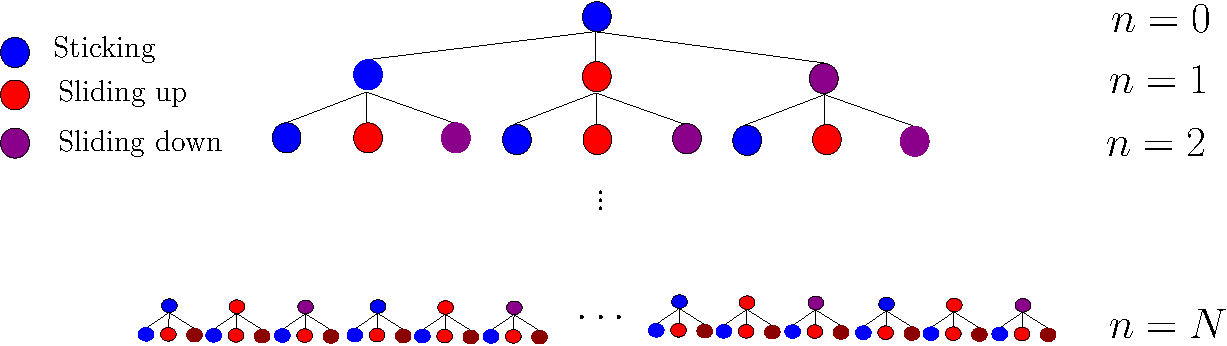
\includegraphics[width=10cm]{MPC_Tree-eps-converted-to.pdf}
\end{center}
\caption[test caption]{\label{fig:mode_tree} \small{Figure from \protect\cite{fom} that represents the exponential growth of the possible modes tree for a single point finger pusher-slider system. The root is a dummy node and, for every other tree level i, each node represents a possible hybrid state for the $i_th$ state transition. Each possible mode can be represented by a path from the root to one of the tree leaves}}
\end{figure}

Using fast iterations of MPC problems to control a hybrid system is a technique used in other robotics fields, as locomotion, and being able to solve them at a frequency high enough to allow direct implementation into a feedback controller design is currently a problem of interest for the robotics community. A proof of this is that in 2016's Workshop on the Algorithmic Foundations of Robotics (WAFR), held in San Francisco last December, Tedrake presented it as one of the current algorithmic open problems in robotics control problems. TODO: Cite

\subsection{Family of Modes} 
\label{subsec:fom}

Responding to the need of obtaining fast solutions to MPC-based control problems Hogan and Rodriguez \cite{fom} proposed an heuristic based procedure to approximately solve them called Family of Modes (FOM). In their work, they assumed a finite horizon MPC problem as the one described in the previous section. At every control step the heuristic method explores the optimization problem over only a small set of all the possible combinations of hybrid states to decide the instantaneous controller policy.

The approximate MPC is characterized by a family of modes, which is defined as the set of modes to consider. If the MPC family contains K modes, the MPC will only solve the K optimization sub-problems resulting when enforcing each mode's hybrid state schedule. The optimal solution is approximated by the best solution between the K considered. This solution will consist of the values of $\diff{\textbf{x}}_i$ and $\diff{\textbf{u}}_i$ for the optimal control trajectory. The controller will then keep executing the first control policy $\textbf{u}_1$ and recomputing the approximate MPC problem frequently to take into account new information as the finite horizon advances in time as well as to tackle external interference with the system and errors in the dynamic model.

In his study, Hogan applied FOM to a system consisting on a single finger point pusher and a square slider and he showed that his method was capable of properly tracking straight line trajectories (and composition of straight lines) under external perturbations by using only three modes. The three modes were selected by hand using intuition on the problem structure. They consisted on exploring the three possible hybrid states (using the notation of section \ref{subsec:frictioncone} they were Sticking, Sliding Right, and Sliding Left) on the first step of the MPC and constraining the system to be in a Sticking state for the rest of the steps.

In this simple case it is possible to derive a good set of modes intuitively, but for more complex and higher dimensional problems, this may not be possible. Furthermore, adding more modes to consider into this heuristic doesn't generally translate into better results and, in some cases, it may lead to results far worse than the original one. For some cases, adding new modes to a family that was able to track a line providing asymptotic convergence could even translate into losing this convergence.

We believe the FOM approach shows promising results and may be able to partially address the current needs of manipulation research to solve the MPC based hybrid control problem. At the same time, we consider necessary to show it's generality and robustness as well as address some of its limitations for it to be adopted in the robotics community.

In the next section we introduce key concepts on sequential properties of heuristic based methods, that will be useful to describe some of the FOM limitations described above. In chapter \ref{sec:goal_revisited} we will revisit the main objectives of our study using the concepts presented in previous sections.

\subsection{Sequential Properties}
\label{subsec:sequential}
On the late 90's, Bertsekas et al. presented a work on the sequential properties of heuristic algorithms \cite{seq}. Two important definitions introduced in their study are sequential consistency and sequential improvement. They also introduce the concept of a roll-out algorithm, which holds a close resemblance to the FOM approach to solve MPC problems. At the end of the section we will further discuss this, but we first need to introduce the main definitions and conclusions of the sequential properties study. We will use the same introductory example used in their study because it is similar to the problem we try to solve. The main differences will be mentioned at the end of the section.

Let us consider a graph search problem on a directed graph with node set N and arc set A. For simplicity, an initial node s is defined. For consistency, we will keep the formulation presented in Bertsekas' study, that groups all the search costs in a subset of terminal (with no outgoing arcs) nodes $\mean{N}$ called destinations. In this formulation, each path from the origin to a destination node $(s, i_1, i_2,..., i_n, \diff{i})$ (see remark \ref{seq_ass}) has an associated cost $g(\diff{i})$ solely defined by the destination node.  We want to find a directed path that starts at the origin s, ends at one of the destination nodes $i \in \mean{N}$, and is such that the cost g(i) is minimized.

\begin{remark} \label{seq_ass}
In order for a sequence $(i_1, i_2,..., i_n)$ to uniquely define the path created by the composition of the arcs $(i_1, i_2), (i_2, i_3),...,(i_{n-1}, i_n)$ we need to assume that given an ordered pair of nodes (i, j), there is at most one arc (i, j) with start node i and end node j. This assumption can always be safely made. 
\end{remark}

\begin{remark} \label{why_terminal_costs}
We allow the node and arc sets, $N$ and $A$, to contain an infinite number of elements. We require, however, that the number of destination nodes be finite.
\end{remark}

The search problem can then be formulated as a DP problem with the nodes corresponding to the states of the DP and the arcs corresponding to the possible state transitions, and the destination nodes corresponding to the terminal states. An heuristic $H$ is then defined as a path construction algorithm that construct a path from a non-destination node to a destination one (remark \ref{path_exists}) and $H(i)$ is defined for any node $i \in N$ as the cost of the destination node of the path constructed by H:
$$ H(i) = g(\diff{i}) $$

\begin{remark} \label{path_exists}
Implicit in this assumption is that for every non-destination node, there exists at least one path starting at that node and ending at some destination node.
\end{remark}

Having introduced this definition of heuristic in this search problem, the concept of roll-out algorithm, first used by Tesauro and Galperin (TODO: Citation) in 1996, is introduced. The formal definition of roll-out algorithm escapes the scope of this study, but an intuitive definition would be:
\begin{definition} \textbf{Roll-out Algorithm:}

Given a starting node s and a heuristic $H$, we define the roll-out algorithm based on $H$ (called $RH$) as following: 
\begin{enumerate}
\item We consider all downstream neighbours i (with $|i| = n$) of s and we apply $H$ at each possible i.
\item We consider the n paths $(i, i_1, ..., \diff{i})$ obtained from the previous step, each of which has an associated cost $H(i)$.
\item We compute the node $i^*$ which minimizes $H(i)$ and we move to the neighbour $i_1^*$.
\item The algorithm is then iteratively developed by considering $i_1^*$ the new start node s and repeating the procedure from step 1 until s is a terminal node.
\end{enumerate}
   
\end{definition}

The nature of the roll-out algorithm and the FOM approach are similar in the sense that use simpler base heuristics that would not give satisfying solutions by themselves and keep applying them at every new step, exploring new paths that were not considered when the heuristics were applied to the root node. This study provided some interesting properties that related the heuristic $H$ with its roll-out $RH$. Most of them were properties that guaranteed that $RH$ would eventually stop (a problem we don't have in our MPC approach, because $|N|$ and $|A|$ are finite) or variations of the roll-out technique that we will discuss later. In order to properly explain them we need to first introduce two main concepts that helped us to understand some of the limitations of the current FOM formulation and that will be discussed on section \ref{subsec:chameleon}. 

\begin{definition} \label{seq_cons} \textbf{Sequential Consistency:}

The heuristic $H$ is said to be sequentially consistent if for every node i, whenever $H$ generates the path $(i, i_1,..., i_m, \diff{i})$ starting at i, it also generates the path $(i_1,..., i_m, \diff{i})$ starting at the node $i_1$.
\end{definition}

\begin{definition} \label{seq_impr} \textbf{Sequential Improvement:}

Suppose that algorithm $H$ generates, starting at each node $i \in N$, a path
$(i, i_1,..., i_m, \diff{i})$ with the property $H(i) \geq H(i_1)$. Then the heuristic H is said to be sequentially improving.

\end{definition}


\begin{figure}[htb!]
\begin{center}
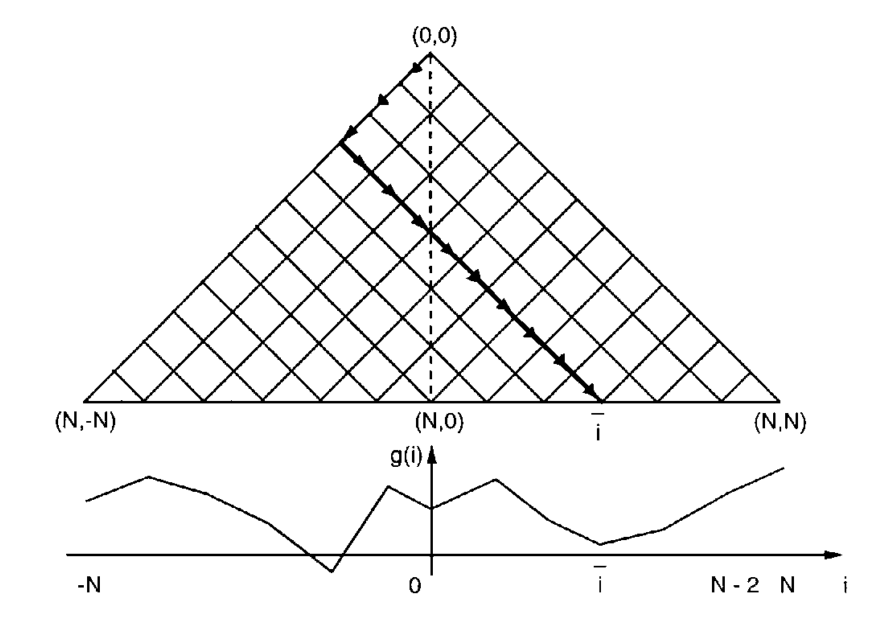
\includegraphics[width=16cm]{seq_cons.png}
\end{center}
\caption{\label{fig:one_d_walk} \small Excerpt from Bertsekas' study. It shows the graph associated with a one dimensional walk problem. The highlighted path corresponds to the result obtained by applying both the roll-out algorithm $RH_1$ from example \ref{one_d_walk_cons}. A plot of the cost function g(i) is shown on the lower part of the picture.}
\end{figure}

We are going to borrow two of Bertsekas' examples (associated with Figure \ref{fig:one_d_walk}) to illustrate this two concepts.

\begin{example} \label{one_d_walk_cons} \textbf{One dimensional walk with a sequentially consistent heuristic:}

Consider a person who walks on a straight line in a temporal and spatial discrete world. During each time step, it can move a fixed length unit to the right or to the left (it cannot stay still). At time 0 this person is at position 0 and it walks for a fixed number of time steps $N$ before ending up in a position $\diff{i} \in [-N, N]$. Each terminal point has an associated cost $g(\diff{i})$ and the objective is to minimize the cost of the terminal position. Figure \ref{fig:one_d_walk} shows a graph representation of the analogue graph search problem, where each node is defined by a state $(k, m)$ where $k$ is the number of steps taken so far and m is the current position. Each node $(k, m)$ has two outgoing arcs: to $(k + 1, m - 1)$ for the left step and to $(k + 1, m + 1)$ for the right one.

Let $H_1$ be an heuristic defined as follows: If $H_1$ applied at node $(k, m)$, it takes $N - k$ successive steps to the right, terminating at the node $(N, m + N - k)$. Note that $H_1$ clearly is sequentially consistent.

The algorithm $RH_1$ applied at node $(k, m)$ uses the roll-out algorithm described above and obtains the path highlighted in Figure \ref{fig:one_d_walk}. In Bertsekas' study it is further proven that the obtained result is always a local minimum.

\end{example}

\begin{example}
Consider the set-up of example \ref{one_d_walk_cons}, and let $H_2$ be defined as follows: when applied at node $(k,m)$, $H_2$ compares the cost $g(m + N - k)$ (corresponding to taking all of the remaining $N - k$ steps to the right) and the cost $g(m - N + k)$ (corresponding to taking all of the remaining $N - k$ steps to the left). If the first is lower, it takes one step to the right. Otherwise, it takes one step to the left. In Bertsekas' work it is mentioned that $H_2$ has no sequential consistency propriety, but has instead sequential improvement. It is also shown that $RH_2$ obtains the global minimum.
\end{example}

Using these definitions, Bertsekas et al. derive some relations between the base heuristics and their associate roll-out procedure. In section \ref{subsec:chameleon} we propose a method to guarantee the sequential improvement of the FOM method when used with a full horizon instead of a finite one. Our method was inspired in a modification of the traditional roll-out technique proposed by Bertsekas called optimal roll-out.

Consider that at a given roll-out step, the heuristic $H$ generates the optimal path $(i_0, i_1,..., i_m, \diff{i})$. Then the fortified roll-out algorithm stores the maximal suffix $S_0 = (i_1, ..., i_m, \diff{i}$ and, in the next roll-out iteration, it will consider the paths generated by $H$ together with the path defined by $S_0$. If the optimal path given by $H$ is not better than the one provided by $S_0$, the algorithm executes the next step of $S_0$ and stores the next maximal suffix $S_1 = (i_2, ..., i_m, \diff{i}$. If the path provided by $H$ is better, its first step is executed and the algorithm stores its maximal suffix. This procedure is followed until reaching one of the terminal nodes.

The main idea behind this modified roll-out technique is to simply keep comparing all the possible paths at a certain step with the best path from the previous step. This way the sequential improvement of the algorithm is clearly guaranteed.

\section{Goal Revisited}
\label{sec:goal_revisited}

To solve MPC problems fast enough to implement them online in a control problem is an open problem of interest for the robotics manipulation community, as explained in section \ref{subsec:MPC}. We consider that Hogan's work in the FOM technique is a good way to provide an heuristic-based approximate solution to this problem. The main objective of this study is to bring this method close to the research community by:
\begin{enumerate}
\item {\textbf{Improving the properties of FOM:}} In section \ref{subsec:chameleon} we will discuss some of it's sequential weaknesses and the solutions we provided and in section \ref{subsec:dynfom} we will present a new FOM-based method to track complex trajectories.

\item{\textbf{Comparing it to other techniques:}} In section \ref{subsec:miqp} we will discuss some of the difficulties we found while trying to compare it to MIQP and we present a modified version of the method to address this problem.

\item{\textbf{Providing a systematic set-up:}} In chapter \ref{sec:modeselection} we will present a systematic protocol with an stochastic approach to choose the modes of the family.

\item{\textbf{Showing the system scalability and robustness:}} We want to track more complex trajectories, more complex systems, and use models of a simple system to solve a problem that uses a more complex one. This study contains results for some of these studies, and they will be discussed through chapters \ref{sec:sim} and \ref{sec:modeselection}. We will also present the studies and experiments we are currently developing for ISRR in chapter \ref{sec:todo}.
\end{enumerate} 

In order to achieve this goals, we provided quantitative tools to evaluate the obtained trajectories that will be presented in section \ref{subsec:costfunc} and we implemented a general simulation interface (presented in chapter \ref{sec:sim}) that allowed us to easily formulate and solve general trajectories and hybrid systems.

The formulation used in our study will be presented in the next chapter, together with all its required theoretic concepts.

\section{Pusher-Slider Formulation}
\label{sec:formulation}
In this section we are going to show all the necessary steps to formulate the FOM problem for the case of a rectangular pusher slider-system with a single finger point pusher.

\subsection{Nomenclature Summary}
\label{subsec:nomenclature}
\begin{table}[H]
\begin{center}
  \begin{tabular}{| l  c  r |}
    \hline
    Property & Symbol & Value \\ \hline
    Coeff. friction (Pusher-Slider)& $\mu_p$ & 0.3 \\
    Coeff. friction (Slider-Ground)& $\mu_g$ & 0.35 \\
    Mass of the slider (\textit{Kg}) & m & 1.05 \\
    Length of the slider (\textit{m}) & a & 0.09 \\
    Width of the slider (\textit{m}) & b & 0.09 \\
    \hline
  \end{tabular}
  \caption {Properties of the slider and the support surface}
\end{center}
\end{table}


\begin{table}[H]
\begin{center}
  \begin{tabular}{| l c |}
    \hline
    Property & Symbol \\ \hline
    Length of the finite horizon & N \\
    Time step & h \\    
    State cost matrix & \textbf{Q} \\
    Control input cost matrix & \textbf{R} \\    
    Final state cost matrix & $\textbf{Q}_f$ \\    
    \hline
  \end{tabular}
  \caption {MPC variable summary}
\end{center}
\end{table}

\begin{table}[H]
\begin{center}
  \begin{tabular}{| l c |}
    \hline
    Property & Symbol \\ \hline
    Position of the slider's CM & $(x, y)^T$ \\
    Slider orientation & $\theta$ \\
    Slider inertial frame & F \\
    Pusher position in F & $(p_x, p_y)^T$ \\
    Pusher velocity in F & $(v_x, v_y)^T$ \\
    Trajectory state & $\textbf{x} = (x, y, \theta, p_y)^T$ \\
    Control input & $\textbf{u} = (v_x, v_y)^T$ \\
    \hline
  \end{tabular}
  \caption {Pusher-Slider system variable summary}
\end{center}
\end{table}


To derive the motion equations and define the MPC state and controller variables, we are going to use the notation used in \cite{fom}. We will first define an inertial reference frame F centred on the slider center of mass that will move and with it. The pose $\textbf{q}$ of the slider's center of mass  will be defined in a fixed world frame $\textbf{q} = (x, y, \theta)^T$ and the pose \textbf{p} of the pusher will be defined relative to the slider center of mass $\textbf{p} = (p_x, p_y)^T$ as shown in Figure \ref{fig:inertial_frame}. The state variable used to define a trajectory is \textbf{x} = $(x, y, \theta, p_y)^T$ and the control input is the velocity of the pusher defined in the center of mass frame $\textbf{u} = \textbf{v}_p = (v_x, v_y)^T$.

\begin{figure}[htb!]
\begin{center}
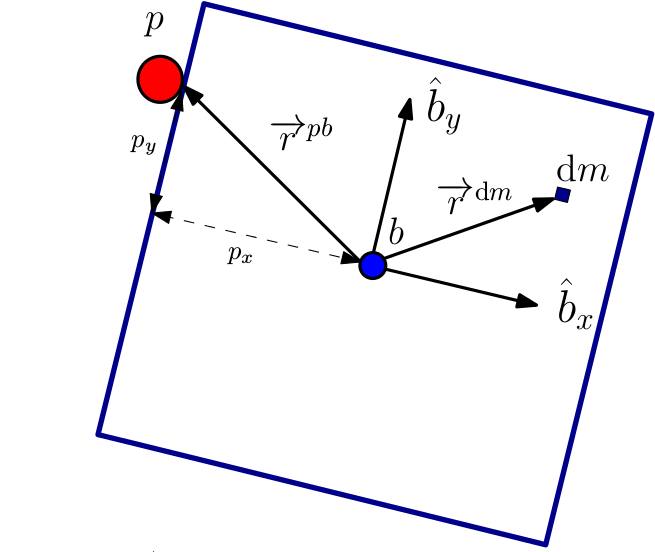
\includegraphics[width=10cm]{inertial_frame.png}
\end{center}
\caption[test caption]{\label{fig:inertial_frame} \small{Figure from \protect\cite{fom} that shows the inertial frame used to define some of the state variables}}
\end{figure}

When talking about hybrid states and modes, we will usually use the following naming convention:
\begin{itemize}
\item {$S$:} Sticking State.
\item {$R$:} Sliding Right State.
\item {$L$:} Sliding Left State.
\item {$\textbf{S}^N$:} Mode defined by $N$ $S$ states $(S, \stackrel{N}{\cdots}, S)$.
\item {$\textbf{R}_i^N$:} Mode defined by $N - 1$ states $S$ and one state $R$ in position $i$. For example, $\textbf{R}_1^3 = (R, S, S)$.
\item {$\textbf{L}_i^N$:} Analogue to $\textbf{R}_i^N$. Mode defined by $N - 1$ states $S$ and one state $L$ in position $i$.
\end{itemize}

\subsection{Quasistatic Pushing Formulation}
\label{subsec:quasistatic}
Quasistatic analysis consists in assuming balance among contact wrenches, gravitation and other applied forces, while neglecting inertial wrenches. This analysis is often taken in manipulation problems, where the trajectory tracking speed changes don't incur into high inertial forces.

The slider of our pusher-slider system with a single finger point pusher is affected by two wrenches: the wrench the pusher applies on the slider ($\textbf{f}_p$) and the wrench the support surface applies to it ($\textbf{f}_g$). Under the quasistatic assumption $\textbf{f}_p = -\textbf{f}_g$.

This assumption will reduce the dimension of the state variables in the motion equations derived in section \ref{subsec:motion_equations} and will allow as to ignore considering a separation hybrid state in our hybrid model of the pusher slider system (if inertial forces were non-negligible the slider could separate away from the pusher while tracking complex trajectories with points of high curvatures). Furthermore, combining the quasistatic assumption with the limit surface of the slider-ground contact, we can derive velocity based motion equations and friction constraints, as will be shown in section \ref{subsec:motion_equations}. The robot arms we had available for this study are velocity-controlled, so this formulation simplifies the experimental implementation of the controller.

\subsection{Ellipsoidal Approximation Of The Limit Surface}
Given a pressure distribution, the associated surface distribution can be numerically computed. Unluckily, the pressure distribution is usually not known exactly and changes over time. For our this study we will assume that the slider and the supporting surface are completely flat, providing a uniform pressure distribution, so $f_n = \dfrac{g m}{A}$, where $f_n$ is the magnitude of the normal support force the ground exerts on the slider and m and A are the slider mass and area, respectively. Furthermore, we will use an approximation to the actual limit surface proposed by Lee and Cutkosky on 1991 \cite{ellipsoidal_ls} based on a study made on 1988 by Howe, Kao, and Cutkosky that showed the suitability of using an elliptic approximation for dry Coulomb friction \cite{elliptical_approx}. We will add further simplifications to their ellipsoid derivation. For a single contact point, their derivation can be simplified, as the limit surface will already be oriented in the ellipsoid major axis. Assuming uniform pressure distribution also simplifies their computation of the maximum momentum around the instantaneous center of rotation. The final procedure to obtain the LS ellipsoid is as follows:

\begin{enumerate}
\item Compute the maximum momentum value. This occurs when the object is in pure rotation, so we can use equation \ref{eq:momentum_cor} considering $\textbf{r}_{IC}$ to be the center of mass (CM) of the slider:
\begin{equation} \label{eq:max_momentum}
n_{max} =  \left| - \mu \, sign(\dot{\theta}) \int_F \textbf{r} \cdot \dfrac{\textbf{r} - \textbf{r}_{CM}}{|\textbf{r} - \textbf{r}_{CM}|} p(\textbf{r}) dA \right| = \mu \dfrac{g m}{A} \int_F ||\diff{\textbf{r}}|| dA
\end{equation}
where $\diff{\textbf{r}}$ is the vector from $\textbf{r}_{CM}$ to \textbf{r}. This gives us the value of the moment semi-axis (the maximum and minimum values of m in the ellipse are going to be $\pm n_{max}$).
\item Similarly, to obtain the force semi-axes, we need the maximum force in the x and y directions, which is going to be $f_{max} = f_n$.
\item The final expression for the ellipsoid is:
\begin{equation} \label{eq:max_momentum}
\left(\dfrac{f_x}{f_{max}}\right)^2 + \left(\dfrac{f_y}{f_{max}}\right)^2 + \left(\dfrac{n}{n_{max}}\right)^2 = 1
\end{equation}
\end{enumerate}


\begin{figure}[htb!]
\begin{center}
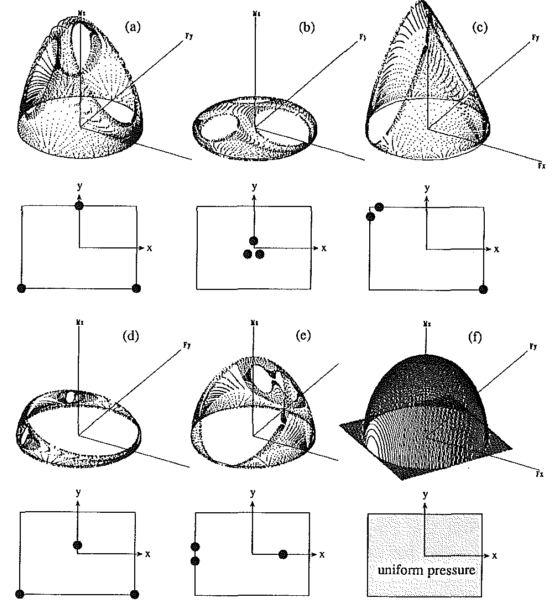
\includegraphics[width=10cm]{ell_limit_surfaces.png}
\end{center}
\caption[test caption]{\label{fig:ls_ellipsoid} \small{Figure from \protect\cite{ellipsoidal_ls} that shows the experimental limit surface for different contact assumptions (that result in different pressure distributions). For the uniform pressure distribution the ellipsoidal approximation describes accurately the LS}}
\end{figure}

\subsection{Motion Cone}
In Hogan's study, a velocity controlled pusher was used. For this reason the motion equations for the MPC problem were formulated in the velocity space. For the case of a single point finger pushing, we can obtain an expression for the friction cone in the velocity space called motion cone (MC) \cite{pushing4} that will be useful to formulate the motion equations and the friction constraints.

As opposed to friction cone, the motion cone is not symmetric with respect to the normal of the contact surface at the point of contact. The cone can be determined by using two angles $\gamma_{t}(\textbf{p})$ and $\gamma_b(\textbf{p})$. Using the ellipsoidal approximation of the LS, the expression of the motion cone for flat sliders can be given as:

\begin{equation}
\gamma_t = \dfrac{\mu_p c^2 - p_x p_y + \mu_p p_x^2}{c^2 + p_y^2 - \mu_p p_x p_y}
\end{equation}
\begin{equation}
\gamma_b = \dfrac{-\mu_p c^2 - p_x p_y - \mu_p p_x^2}{c^2 + p_y^2 + \mu_p p_x p_y}
\end{equation}
where $p_x$ and $p_y$ have been defined in section \ref{subsec:nomenclature} and $c = \dfrac{f_{max}}{n_{max}}$.

\begin{figure}[htb!]
\begin{center}
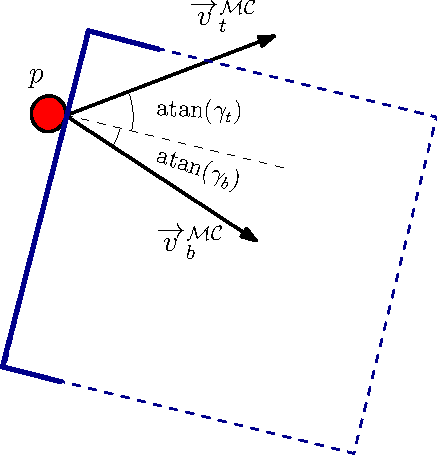
\includegraphics[width=7cm]{MotionCone-eps-converted-to.pdf}
\end{center}
\caption[test caption]{\label{fig:motion_cone} \small{Figure from \protect\cite{fom} with a representation of the motion cone}}
\end{figure}

We will define $\gamma := \dfrac{v_y}{v_x}$. If the velocity vector lies inside the motion cone, the pusher will stick. If $\gamma > \gamma_t$ the slider will slip to the right with respect to the pusher. Finally, if $\gamma < \gamma_b$ the slider will slip to the left with respect to the pusher. In summary the friction constraints can be expressed for each hybrid state as:

\begin{equation} \label{eq:sticking_cone}
\textbf{Sticking:}\,\,\,\,\, \textbf{u} \in MC: 
			\begin{cases}
               v_y \leq \gamma_t v_x\\
               v_y \geq \gamma_b v_x\\
            \end{cases}
\end{equation}

\begin{equation}\label{eq:right_cone}
\textbf{Sliding Right:}\,\,\,\,\, \textbf{u} > MC: v_y > \gamma_t v_x            
\end{equation}

\begin{equation}\label{eq:left_cone}
\textbf{Sliding Left:}\,\,\,\,\, \textbf{u} < MC: v_y < \gamma_b v_x
\end{equation}

TODO: Decide what to do with Maria's piece of advice on these equations.

In our single finger point pusher system the three possible hybrid states of the system will be these. The quasistatic assumption guarantees that the slider doesn't move away from the pusher by virtual inertial forces and we will impose constraints on the pusher to prevent it to move away from the slider: the normal velocity of the pusher with respect to the contact surface will be non-negative and the tangential displacement from the contact surface center ($p_y$) will be constrained to prevent the pusher from slipping through the slider sides.

\subsection{Motion Equations} \label{subsec:motion_equations}
The motion equations are adapted from the ones used in Hogan's work. They were originally inspired in a pusher-slider system study by Lynch et al. \cite{motion_equations} and can be expressed as follows:

(TODO: Should I add the derivation from Lynch?)

\begin{equation} \label{eq:motion_equation}
\dot{\textbf{x}} = \begin{cases}
					f_1(\textbf{x}, \textbf{u}) \,\, \text{if \textbf{u} $\in$ MC} \\
					f_2(\textbf{x}, \textbf{u}) \,\, \text{if \textbf{u} $>$ MC} \\
					f_3(\textbf{x}, \textbf{u}) \,\, \text{if \textbf{u} $<$ MC}
\end{cases}
\end{equation}
\begin{equation}
f_i(\textbf{x}, \textbf{u}) = 
\begin{pmatrix} 
	\textbf{CQP}_i \\ 
	\textbf{b}_i \\
	\textbf{c}_i 
\end{pmatrix} \textbf{u} := \hat{\textbf{B}}_j(\textbf{x})\cdot\textbf{u}
\end{equation}
where 
$\textbf{C} = \begin{pmatrix} 
cos(\theta) & -sin(\theta) \\
sin(\theta) & cos(\theta)
\end{pmatrix}
$ \,\,\,\, and  \,\,\,\,
$\textbf{Q} = \dfrac{1}{c^2 + p_x^2 + p_y^2} \begin{pmatrix} 
c^2 + p_x^2 & p_x p_y \\
p_x p_y & c^2 + p_y^2
\end{pmatrix}$. \\ \\
$\textbf{P}_i$, $\textbf{b}_i$ and $\textbf{c}_i$ are mode-dependant matrices and take the following values: \\ \\
$\textbf{b}_1 = \dfrac{1}{c^2 + p_x^2 + p_y^2} \begin{pmatrix} -p_y & p_x \end{pmatrix}$, \,$\textbf{b}_2 = \dfrac{1}{c^2 + p_x^2 + p_y^2} \begin{pmatrix} -p_y + \gamma_t p_x & 0 \end{pmatrix}$, \,$\textbf{b}_3 = \dfrac{1}{c^2 + p_x^2 + p_y^2} \begin{pmatrix} -p_y + \gamma_b p_x & 0 \end{pmatrix}$ \\ \\
$\textbf{c}_1 = \begin{pmatrix}
0 & 0
\end{pmatrix}$,\,\,\,\,\,\,\,\,\,\,\,\,\,\,\,\,\,\,\,\,\,\,\,\,\,\,\,\,\,\,\,\,\,\,\,\,\,\,\,\,\,\,\,\,\,\,
$\textbf{c}_2 = \begin{pmatrix}
-\gamma_t & 1
\end{pmatrix}$,\,\,\,\,\,\,\,\,\,\,\,\,\,\,\,\,\,\,\,\,\,\,\,\,\,\,\,\,\,\,\,\,\,\,\,\,\,\,\,\,\,\,\,\,\,\,\,\,\,\,\,\,\,\,\,
$\textbf{c}_3 = \begin{pmatrix}
-\gamma_b & 1
\end{pmatrix}$ \\ \\
$\textbf{P}_1 = \begin{pmatrix}
1 & 0 \\ 0 & 1
\end{pmatrix}$, \,\,\,\,\,\,\,\,\,\,\,\,\,\,\,\,\,\,\,\,\,\,\,\,\,\,\,\,\,\,\,\,\,\,\,\,\,\,\,  $\textbf{P}_2 = \begin{pmatrix}
1 & 0 \\ \gamma_t & 0
\end{pmatrix}$, \,\,\,\,\,\,\,\,\,\,\,\,\,\,\,\,\,\,\,\,\,\,\,\,\,\,\,\,\,\,\,\,\,\,\,\,\,\,\,\,\,\,\,\,\,\,\,\,\,\,\,\,\,  $\textbf{P}_3 = \begin{pmatrix}
1 & 0 \\ \gamma_b & 0
\end{pmatrix}$ \\ \\
where i = 1, 2, 3 correspond to the states of Sticking, Sliding Right and Sliding Left respectively. For simplicity, we do not consider a state where the pusher is separated from the slider for the controller modelling. In the controller we impose constraints that forbid the pusher to move outside of the slider side borders and the under the quasistatic assumption, the slider will not separate from the pusher by it inertia.

On the other hand the possibility of separation is included in the simulator, in order to represent the experimental set-up more accurately and to detect possible errors in the controller design.

The motion equations are going to be used to define constraints in the MPC problem and, in turn, the MPC formulation is going to be fed into a commercial optimizer to obtain the optimal values of \textbf{x} and \textbf{u} that fulfil all the constraints. The fact that the motion equations are nonlinear would require using a nonlinear optimizer, which would represent too much computational cost to solve the problem online at every control iteration. In order to obtain a more tractable formulation the motion equations will be linearized around a nominal trajectory $\textbf{x}^*(t)$ and control input $\textbf{u}^*(t)$. We will use $(.)^*$ to denote elements of the nominal problem and $\diff{(.)}$ to denote perturbations around the nominal value. Using this notation, the linearization of the motion equation \ref{eq:motion_equation} is:
\begin{equation} \label{eq:condensed_motion_linear}
\dot{\diff{\textbf{x}}} = \textbf{A}_i(\textbf{x}^*, \textbf{u}^*)\cdot \diff{\textbf{x}} + \textbf{B}_i(\textbf{x}^*, \textbf{u}^*)\cdot \diff{\textbf{u}} + f_i(\textbf{x}^*, \textbf{u}^*) - \dot{\textbf{x}}^*
\end{equation}
$\textbf{A}_i(\textbf{x'}, \textbf{u'}) = \left.\dfrac{\partial f_i(\textbf{x}, \textbf{u})}{\partial \textbf{x}}\right|_{\textbf{x'}, \textbf{u'}}$, $\textbf{B}_i(\textbf{x'}, \textbf{u'}) = \left.\dfrac{\partial f_i(\textbf{x}, \textbf{u})}{\partial \textbf{u}}\right|_{\textbf{x'}, \textbf{u'}} = \hat{\textbf{B}}_i(\textbf{x'})$
,with $\diff{\textbf{x}} = \textbf{x} - \textbf{x}^*$ and $\diff{\textbf{u}} = \textbf{u} - \textbf{u}^*$ \\

It should be noted that equation \ref{eq:condensed_motion_linear} is different from the linearized motion equation presented in Hogan's work. This fact will be discussed further in section \ref{subsec:nominal_mode} but the main idea is that the term $f_i(\textbf{x}^*, \textbf{u}^*) - \dot{\textbf{x}}^*$ cannot generally be cancelled as in other traditional control problems because $f_i(\textbf{x}^*, \textbf{u}^*)$ will not describe the instantaneous motion of the nominal trajectory if the nominal trajectory is in a hybrid state different from the one defined by $i$.

Similarly to the linearization of the motion equation, the friction constraint equations from \ref{eq:sticking_cone} to \ref{eq:left_cone} can also be linearized with respect to $\diff{\textbf{x}}$. For consistency with the variables used for the motion equations ($\diff{\textbf{x}}$ and $\diff{\textbf{u}}$) $v_x$ and $v_y$ are expressed as $v_x^* + \diff{v}_x$ and $v_y^* + \diff{v}_y$ respectively:

\begin{equation} \label{eq:sticking_cone_linear}
\textbf{Sticking:}\,\,\,\,\, 
			\begin{cases}
              (v_y^* + \diff{v}_y) \leq (\gamma_t(\textbf{x}^*) + \textbf{C}_t(\textbf{x}^*)\cdot \diff{\textbf{x}})(v_x^* + \diff{v}_x)\\
              (v_y^* + \diff{v}_y) \geq (\gamma_b(\textbf{x}^*) + \textbf{C}_b(\textbf{x}^*)\cdot \diff{\textbf{x}})(v_x^* + \diff{v}_x)\\
            \end{cases}
\end{equation}

\begin{equation}\label{eq:right_cone_linear}
\textbf{Sliding Right:}\,\,\,\,\, (v_y^* + \diff{v}_y) > (\gamma_t(\textbf{x}^*) + \textbf{C}_t(\textbf{x}^*)\cdot \diff{\textbf{x}})(v_x^* + \diff{v}_x)            
\end{equation}

\begin{equation}\label{eq:left_cone_linear}
\textbf{Sliding Left:}\,\,\,\,\, (v_y^* + \diff{v}_y) < (\gamma_b(\textbf{x}^*) + \textbf{C}_b(\textbf{x}^*)\cdot \diff{\textbf{x}})(v_x^* + \diff{v}_x)
\end{equation}

where $\textbf{C}_t(\textbf{x'}) = \left.\dfrac{\partial \gamma_t}{\partial \diff{\textbf{x}}}\right|_{\textbf{x'}}$ and $\textbf{C}_b(\textbf{x'}) = \left.\dfrac{\partial \gamma_b}{\partial \diff{\textbf{x}}}\right|_{\textbf{x'}}$


This notation allows us to write all the linearized motion cone constraints in a condensed form suitable for a linear programming optimizer, as equation \ref{eq:condensed_motion_linear}:

\begin{equation} \label{eq:condensed_cone_linear}
\textbf{E}_i(\textbf{x}^*, \textbf{u}^*)\cdot \diff{\textbf{x}} + \textbf{D}_i(\textbf{x}^*)\cdot \diff{\textbf{u}} \leq g_i(\textbf{x}^*, \textbf{u}^*)
\end{equation} \\ \\
$\textbf{E}_1(\textbf{x'}, \textbf{u'}) = v_y' \begin{pmatrix}
-\textbf{C}_t(\textbf{x'}) \\
\textbf{C}_b(\textbf{x'})
\end{pmatrix}$,\,\,\,\,\,\,\,\,\,\,\,\,\,\,\,\,\,\,\,\,\,\,\,\,\,\, $\textbf{E}_2(\textbf{x'}, \textbf{u'}) = v_y' \textbf{C}_t(\textbf{x'})$,\,\,\,\,\,\,\,\,\,\,\,\,\,\,\,\,\,\,\,\,\,\,\,\,\,\,\,\,\,\,\,\,\,\, $\textbf{E}_3(\textbf{x'}, \textbf{u'}) = -v_y' \textbf{C}_b(\textbf{x'})$ \\ \\
$\textbf{D}_1(\textbf{x'}) = \begin{pmatrix}
-\gamma_t(\textbf{x'}) & 1 \\
\gamma_b(\textbf{x'}) & -1
\end{pmatrix}$,\,\,\,\,\,\,\,\,\,\,\,\,\,\,\,\,\,\,\,\,\,\,\,\,\,\,\,\, $\textbf{D}_2(\textbf{x'}) = \begin{pmatrix}
-\gamma_t(\textbf{x'}) & -1
\end{pmatrix}$,\,\,\,\,\,\,\,\,\,\,\,\,\,\,\,\,\,\,\,\,\,\,\,\, $\textbf{D}_3(\textbf{x'}) = \begin{pmatrix}
-\gamma_b(\textbf{x'}) & 1
\end{pmatrix}$ \\ \\
$\textbf{g}_1(\textbf{x'}, \textbf{u'}) = \begin{pmatrix}
-v_y' + \gamma_t(\textbf{x'}) v_x'\\
 v_y' - \gamma_b(\textbf{x'}) v_x'
\end{pmatrix}$,\,\,\,\,\,\,\,\,\,\,\,\,\,\,\,\,\, $\textbf{g}_2(\textbf{x'}, \textbf{u'}) = v_y' - \gamma_t(\textbf{x'}) v_x' - \epsilon$,\,\,\,\,\,\,\,\,\,\,\,\,\,\,\,\, $\textbf{g}_3(\textbf{x'}, \textbf{u'}) = -v_y' + \gamma_b(\textbf{x'}) v_x' - \epsilon$ \\

\begin{remark}
$\epsilon$ is just a small positive scalar used to express strict inequalities, as the optimizer we used only supported non-strict ones.
\end{remark}

\subsection{MPC And MIQP Formulation} \label{subsec:mpc_formulation}

As explained in section \ref{subsec:MPC}, each MPC mode fixed sub-problem will compute the optimal values for the state and control variables for a discrete finite horizon of N steps, a time step h, and a given initial position $\diff{\textbf{x}}_0$ to minimize the cost equation provided in equation \ref{eq:cost_function}, subject to motion and cone constraints. We will use the perturbation dynamics, so the state and control variables will be $(\diff{\textbf{x}}_1, ..., \diff{\textbf{x}}_N)$ and $(\diff{\textbf{u}}_0, ..., \diff{\textbf{u}}_{N-1})$; and the initial state will be $\textbf{x}_0$. As MPC considers a discrete framework, we need to discretize the motion equations from previous section. After a first order discretization, the MPC constraints at step j are:
\begin{equation} \label{eq:mpc_constraints_initial_step}
\text{if } j = 0: \begin{cases}
\diff{\textbf{x}}_1 = \diff{\textbf{x}}_0 +  h \textbf{B}_{i0}(\textbf{x}_0) \cdot \diff{\textbf{u}}_0 + h \textbf{f}_{i0} + \textbf{x}_0^* - \textbf{x}_1^*\\
\textbf{D}_{i0} \cdot \diff{\textbf{u}}_0 \leq \textbf{g}_{i0}
\end{cases}
\end{equation}
\begin{equation} \label{eq:mpc_constraints_non_initial_step}
\text{if } j > 0: \begin{cases}
\diff{\textbf{x}}_{j+1} = (\textbf{I} + h \textbf{A}_{ij})\cdot \diff{\textbf{x}}_j + h \textbf{B}_{ij} \cdot \diff{\textbf{u}}_j + h \textbf{f}_{ij}  + \textbf{x}_{j}^* - \textbf{x}_{j+1}^*\\
\textbf{E}_{ij} \cdot \diff{\textbf{x}}_j + \textbf{D}_{ij} \cdot \diff{\textbf{u}}_j \leq \textbf{g}_{ij}
\end{cases}
\end{equation}
where $\textbf{A}_{ij} = \textbf{A}_i(\textbf{x}_j^*, \textbf{u}_j^*)$, and $\textbf{E}_{ij} = \textbf{E}_i(\textbf{x}_j^*, \textbf{u}_j^*)$, using the notation from section \ref{subsec:motion_equations}. $\textbf{f}_{ij}$ is defined differently depending on the iteration step:
$$ \textbf{f}_{ij} = \begin{cases} \textbf{f}_{i}(\textbf{x}_j, \textbf{u}_j^*)\text{,  \,\,\,\,(if j = 0)} \\
\textbf{f}_{i}(\textbf{x}_j^*, \textbf{u}_j^*) \text{, \,\,\,\,(if j $>$ 0)} 
\end{cases}$$

$\textbf{B}_{ij}$, $\textbf{D}_{ij}$, $\textbf{E}_{ij}$, and $\textbf{g}_{ij}$ are defined in an analogue way, evaluating their section \ref{subsec:motion_equations} counterparts on $\textbf{x}_j$ for the first step and on $\textbf{x}_j^*$ for the following ones.

\begin{remark}
For the case j = 0, $\diff{\textbf{x}}_0$ is known value, so the first order discrete version of equation \ref{eq:motion_equation} becomes:
\begin{equation}
\textbf{x}_1 = \diff{\textbf{x}}_1 + \textbf{x}_1^* = h \textbf{f}_i(\textbf{x}_0, \textbf{u}_0) + \textbf{x}_0 = h \hat{\textbf{B}}_i(\textbf{x}_0)  (\diff{\textbf{u}}_0 + \textbf{u}_0^*) + \diff{\textbf{x}}_0 + \textbf{x}_0^* 
\end{equation}
and by isolating $\diff{\textbf{x}}_1$ we can obtain the linear motion equation in expression \ref{eq:mpc_constraints_initial_step} without having to apply a linearization step. In a similar way, the friction constraints can also be expressed as linear constraints with respect to $\diff{\textbf{u}}_0$ 
\end{remark}

Let $m = (s_0, ..., s_N)$ denote the hybrid mode where at step j of the fixed mode MPC sub-problem the system is in the hybrid state $s_j$. Then, the sub-problem constraints are formulated by substituting i with $s_j$ in equations \ref{eq:mpc_constraints_initial_step} and \ref{eq:mpc_constraints_non_initial_step}. Then the optimization problem is fed into the commercial optimizer Gurobi \cite{gurobi} to obtain the optimal values of $(\diff{\textbf{x}}_1, ..., \diff{\textbf{x}}_N)$ and $(\diff{\textbf{u}}_0, ..., \diff{\textbf{u}}_{N-1})$, together with the optimal cost function. The full MPC problem solution is then approximated to be the best sub-problem solution.

As will be explained in section \ref{subsec:miqp}, we also implemented an MIQP solver to compare our FOM against. The formulation we have presented in this section has already linear constraints and quadratic cost function, so we can apply quadratic programming solvers to them. Gurobi allowed us to formulate the mode dependent constraints by using binary decision variables and a big-M notation. The resulting formulation for the motion and friction constraints is as follows: 
\begin{equation} \label{eq:big_m_first_step}
\text{if } j = 0: \begin{cases}

\textbf{x}_1 \leq (\diff{\textbf{x}}_0 +  h \textbf{B}_{i0}(\textbf{x}_0) \cdot \diff{\textbf{u}}_0 + h \textbf{f}_{i0} + \textbf{x}_0^* - \textbf{x}_1^*) + M (1 - z_{i0})\\

-\textbf{x}_1 \leq -(\diff{\textbf{x}}_0 +  h \textbf{B}_{i0}(\textbf{x}_0) \cdot \diff{\textbf{u}}_0 + h \textbf{f}_{i0} + \textbf{x}_0^* - \textbf{x}_1^*) + M (1 - z_{i0})\\

\textbf{D}_{i0} \diff{\textbf{u}}_0 \leq \textbf{g}_{i0} + \textbf{1}_{2\times1}M(1 - z_{i0})
\end{cases}
\end{equation}
\begin{equation} \label{eq:big_m_other_steps}
\text{if } j > 0: \begin{cases}

\diff{\textbf{x}}_{j+1} \leq [(\textbf{I} + h \textbf{A}_{ij})\cdot \diff{\textbf{x}}_j + h \textbf{B}_{ij} \cdot \diff{\textbf{u}}_j + h \textbf{f}_{ij}  + \textbf{x}_{j}^* - \textbf{x}_{j+1}^*] + M(1-z_{ij})\\

-\diff{\textbf{x}}_{j+1} \leq -[(\textbf{I} + h \textbf{A}_{ij})\cdot \diff{\textbf{x}}_j + h \textbf{B}_{ij} \cdot \diff{\textbf{u}}_j + h \textbf{f}_{ij}  + \textbf{x}_{j}^* - \textbf{x}_{j+1}^*] + M(1-z_{ij})\\

\textbf{E}_{ij} \diff{\textbf{x}}_j + \textbf{D}_{ij} \diff{\textbf{u}}_j \leq \textbf{g}_{ij} + \textbf{1}_{2\times1}M(1 - z_{ij})
\end{cases}
\end{equation}
\begin{equation} \label{eq:binary_const}
z_{1j} + z_{2j} + z_{3j} = 1
\end{equation}

The equality constraints $a = b$ (where a and u are functions of \textbf{x} and \textbf{u}) have been broken into two inequality ones $a \leq b$ and $-a \leq -b$ and each mode independent constraint $a \leq b$ has been modified into $a \leq b + M(1 - z_{ij})$ for an appropriate binary variable $z_{ij}$. If the sub-problem is in state i at step j, $z_{ij}$ = 1 and the term $M(1 - z_{ij})$ is zero and the original inequality constrains applies. If the sub-problem is not in that state at step j, $z_{ij}$ = 0 and the inequality becomes $a \leq b + M$. If the value of M is high enough (specifically, if it is higher than any possible value of the expression a - b) the inequality becomes redundant. Equation \ref{eq:binary_const} enforces that the MPC sub-problems are in one and only one hybrid state at each step.

\section{Simulation Interface}
\label{sec:sim}

The simulations of Hogan's study were mainly designed for an specific choice of modes and a specific trajectory to follow. In this study, we wanted to study general properties of the FOM problem, to generalize the results to more complex pusher-slider systems and trajectories, and to compare our different FOM strategies to solve the MPC problem with other conventional methods as MIQP. In order to satisfy this needs, we decided to implement a general simulation tool. The code main structure can be described as follows:

An abstract state interface is implemented to provide the dynamics and cone constraints of the state as well as their linearized versions at a certain objective state space and control input. To define a certain experimental problem, the dynamics function and constraint equations are derived depending on a general state space variable \textbf{x} and controller action \textbf{u} and the necessary state instances are implemented and a mode is then defined by a vector of state handles. An MPC solver class it's also implemented to get an initial condition and an objective trajectory and return a control input. Each MPC solver implementation can include its own member states or modes (as well as other optimization set-up variables) and internally decides how to handle them.

At the same time, an Euler integration simulator is implemented. This simulator uses it's own state classes to describe the dynamics of the pusher slider system. These states are independent from the optimization ones so that discrepancies between model and reality can be simulated (for example the MPC solver can use linearized dynamics or cone constraints while the Euler integrator uses the non-linearized version, which is more similar to the real experimental set-up than using linearized dynamics in both places). The Euler integration class also holds a member MPC solver that returns the control input to be applied. The integrator then computes the value of the state variable derivative $\dot{x}$ and uses a simple quadrature to approximate the next state variable value.

The controller (MPC solver) and simulator are decoupled, so they can consider different hybrid states. This allows us to consider more realistic models for the euler integration step of the simulation (we always use non-linearized motion equations for the integration step), to use different parameters in their states (to test controllers designed for a certain slider shape, $\mu_g$, and $\mu_p$ together with a simulator set-up with different parameters, to show the robustness of the controller to uncertainties in the models).

\subsection{Local, Global and MPC Costs}
\label{subsec:costfunc}
During the previous work at MCubelab, there was no systematic and objective way to evaluate the global trajectory resulting from the FOM control law, the exit or failure of an experiment was mainly determined in a subjective binary way. If the pusher slider didn’t show appreciable divergence (at the naked eye) from the planned trajectory it was considered a success, otherwise it was a failure. In a similar fashion if the system was perturbed (by an external interaction), the success lied in recovering the original trajectory in a “reasonable” time determined subjectively. The main goal of the study was just to demonstrate that FOM could effectively control the pusher slider system to track previously planned trajectories, and that all this process could be done online. Because of this proof-of-concept nature, this approach was sufficient.

For this thesis we wanted a more objective way to evaluate how good a control trajectory was and this required a certain notion of metric or score for the global trajectory. We tried to keep coherence between the global and local cost functions, but removed the $\diff{\textbf{x}}_N^T \textbf{Q}_{f}^{} \diff{\textbf{x}}_N^{}$ term of the cost function. As presented in section \ref{subsec:MPC}, this term is used to account for the information missing because of the finite horizon. When scoring the final trajectory, we have the full horizon information, so this term is no longer required. The obtained cost function is $S = \sum\limits_{i = 0}^{M}(\diff{\textbf{x}}_{i}^{T} \textbf{Q} \diff{\textbf{x}}_i^{} + \diff{\textbf{u}}_{i}^{T} \textbf{R} \diff{\textbf{u}}_i^{})$, where $M$ is the number of euler integration steps. We will denote by local cost over time each of the $\diff{\textbf{x}}_{i}^{T} \textbf{Q} \diff{\textbf{x}}_i^{} + \diff{\textbf{u}}_{i}^{T} \textbf{R} \diff{\textbf{u}}_i^{}$ values.

It is important to note that even if this global cost function is used score how close the obtained trajectory was from the desired one, it is not a direct indicator of the MPC solving performance. We will denote the cost function provided in section \ref{subsec:MPC} as MPC cost. Then optimizing the MPC cost at each iteration could incur in a larger optimal cost for the global trajectory. If we are currently at the state $x_i$ and we consider two modes $M_1$ and $M_2$ with local costs $c_1$ and $c_2$, with $c_1 < c_2$ there's no guarantee that executing the first step of the trajectory obtained from mode $M_1$ will translate in a smaller global cost function. Some causes for this effect are exposed and fixed in \ref{subsec:chameleon} but, even after fixing them and considering an ideal world scenario (where the models are completely accurate and there's no sensor noise), the fact that the receding finite horizon adds new information to the problem at every control iteration implies that the optimal state and control pair $(x_{i+1}, u_{i})$ computed at the control iteration $i$ could technically lose their optimal property when the information from control iteration $i+1$ is introduced.

This effect is common in all receding finite horizon problems and there's usually no way to completely solve it. In order to evaluate the MPC solving performance of our method, some of the simulation results we expose in the following sections show a plot of the local MPC cost over time in addition to a graphical representation of the trajectory and it's global or local cost. It will be shown that, when extending a family $F_1$ into a family $F_2$ by adding more modes, the local cost of $F_2$ descends with respect ot $F_1$ in the first bifurcation of the local MPC cost over time plot. This will be further discussed in section \ref{subsec:simresults}.

\subsection{Nominal Mode}
\label{subsec:nominal_mode}
In section \ref{subsec:motion_equations} we noted that, as opposed to the previous study, we do not simplify the term $f_i(\textbf{x}^*, \textbf{u}^*) + \dot{\textbf{x}}^*$ in equation \ref{eq:condensed_motion_linear}. $\textbf{x}^*$ can be described by the same motion equations as $\textbf{x}$ using the hybrid state friction constraints to determine the hybrid state, but it is important to realize that, once we constrain out system to be in a state $i$ at a time instant $t_j$, the specific motion equation that describes this instant-state system $f_i(\textbf{x}_j, \textbf{u}_j)$ may not describe the instantaneous motion of the nominal trajectory. The nominal trajectory will clearly be described by $f_{i'}(\textbf{x}_j^*, \textbf{u}_j^*)$, but there's no guarantee that $i = i'$. The error introduced by assuming $f_i(\textbf{x}^*, \textbf{u}^*) + \dot{\textbf{x}}^* = 0$ can be critical for the performance of the controller. In Figure \ref{fig:without_nominal_trajectory} we can see the behaviour of the FOM approach when trying to track a circle using a family of modes learned using the procedure described in section \ref{subsec:learningsimple}. The red slider follows the nominal trajectory. The trajectory followed by its center of mass trajectory is represented with the black line. The blue slider follows the simulated trajectory and its center of mass follows the blue line. The last position of the simulated slider is highlighted and the other snapshots are faded away. The considered optimal paths the MPC considers are shown at the center of each simulated slider. The chosen path is the yellow one. As can be seen the obtained trajectory diverges from the nominal one. Furthermore, it can be seen how the optimal finite horizon trajectory computed in the MPC problem is completely different from the realized trajectory. In Figure \ref{fig:without_nominal_local_cost} the correspondent local cost over time is shown.

\begin{figure}[htb!]
\begin{center}
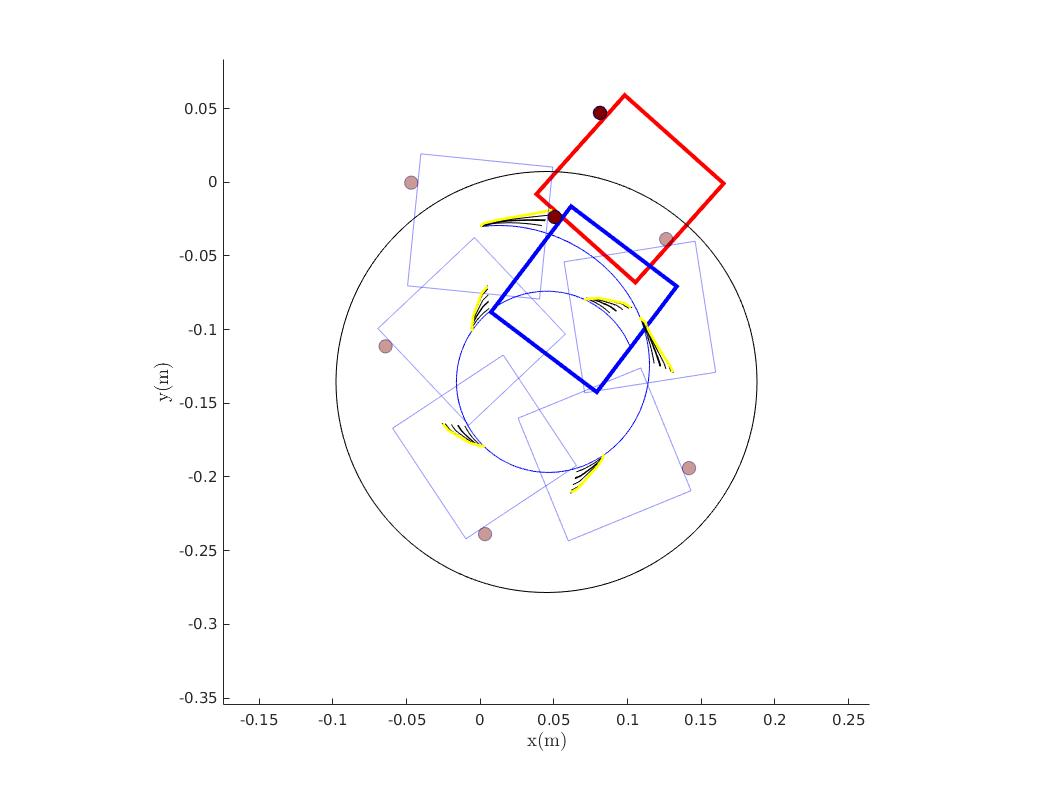
\includegraphics[width=16cm]{without_nominal_trajectory.jpg}
\end{center}
\caption{\label{fig:without_nominal_trajectory} \small Snapshot from the video simulating the trajectory obtained when tracking a circular trajectory with the 8 best modes obtained using section \ref{subsec:learningsimple} procedure.}
\end{figure}

\begin{figure}[htb!]
\begin{center}
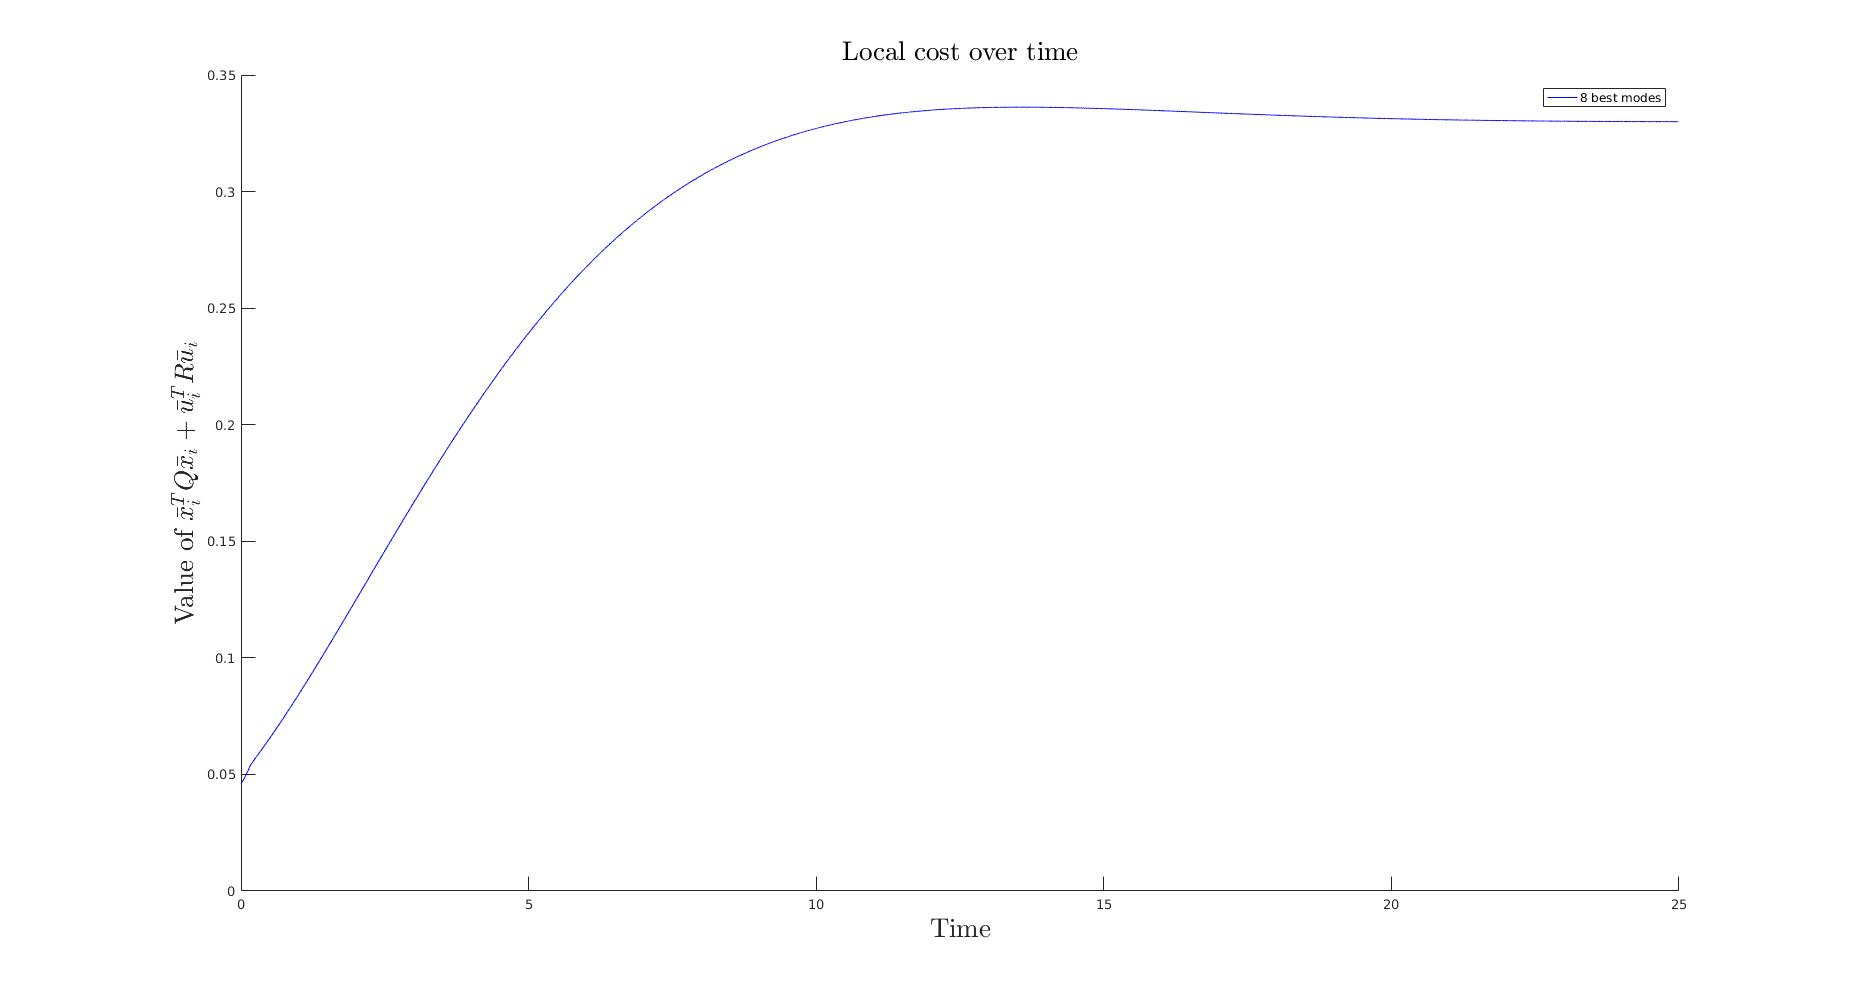
\includegraphics[width=16cm]{without_nominal_local_cost.jpg}
\end{center}
\caption{\label{fig:without_nominal_local_cost} \small Local cost over time associated to the trajectory in Figure \ref{fig:without_nominal_trajectory}}
\end{figure}

The possibility of the hybrid states associated the nominal trajectory to be different from the ones associated with the real trajectory has another important implication. The perturbation state motion equation \ref{eq:condensed_motion_linear} has the nominal trajectory as an equilibrium point only when $i = i'$. Otherwise, if we consider $\textbf{x} = \textbf{x}^*$ and $\textbf{u} = \textbf{u}^*$, we obtain $\diff{\textbf{x}} = \textbf{A}_i \cdot \textbf{0} + \textbf{B}_i \cdot \textbf{0} + f_i(\textbf{x}^*, \textbf{u}^*) - \dot{\textbf{x}}^* = f_i(\textbf{x}^*, \textbf{u}^*) - f_{i'}(\textbf{x}^*, \textbf{u}^*)$. If none of the MPC modes is the one that the nominal trajectory follows, the solution $\diff{\textbf{x}}_j = \diff{\textbf{u}}_j = \textbf{0}$ will never be feasible, and we will never be able to stabilize the planned trajectory on the nominal one, even if the initial state is on the nominal trajectory ($\textbf{x}_0 = \textbf{0}$). In order to force the MPC to consider the nominal mode, we can simply compute it at every MPC step (it can be easily determined applying the friction constraints to each pair $\textbf{x}_j^*$, $\textbf{u}_j^*$) and add it as one of the modes of the family.

\subsection{Chameleon Mode}
\label{subsec:chameleon}

In the previous FOM study there was no guarantee of improvement in the obtained trajectory by considering new modes in a previously used family. It needs to be clarified that, even if in the previous study there was no global score function implemented, this effect could be so big that it could be observed with the naked eye. An illustrative example would be the following. A family containing only the sticking mode $F_1 = \textbf{S}$ would greatly outperform the extended family $F_2 = \textbf{S} \cup (L, R, S, \stackrel{N-2}{\cdots}, S)$. On the other side a further extension $F_3 = F_2 \cup \textbf{R}_1$ would outperform the two previous families. This behaviour can be shown in Figure \ref{fig:non_chameleon}.

\begin{figure}[htb!]
\begin{center}
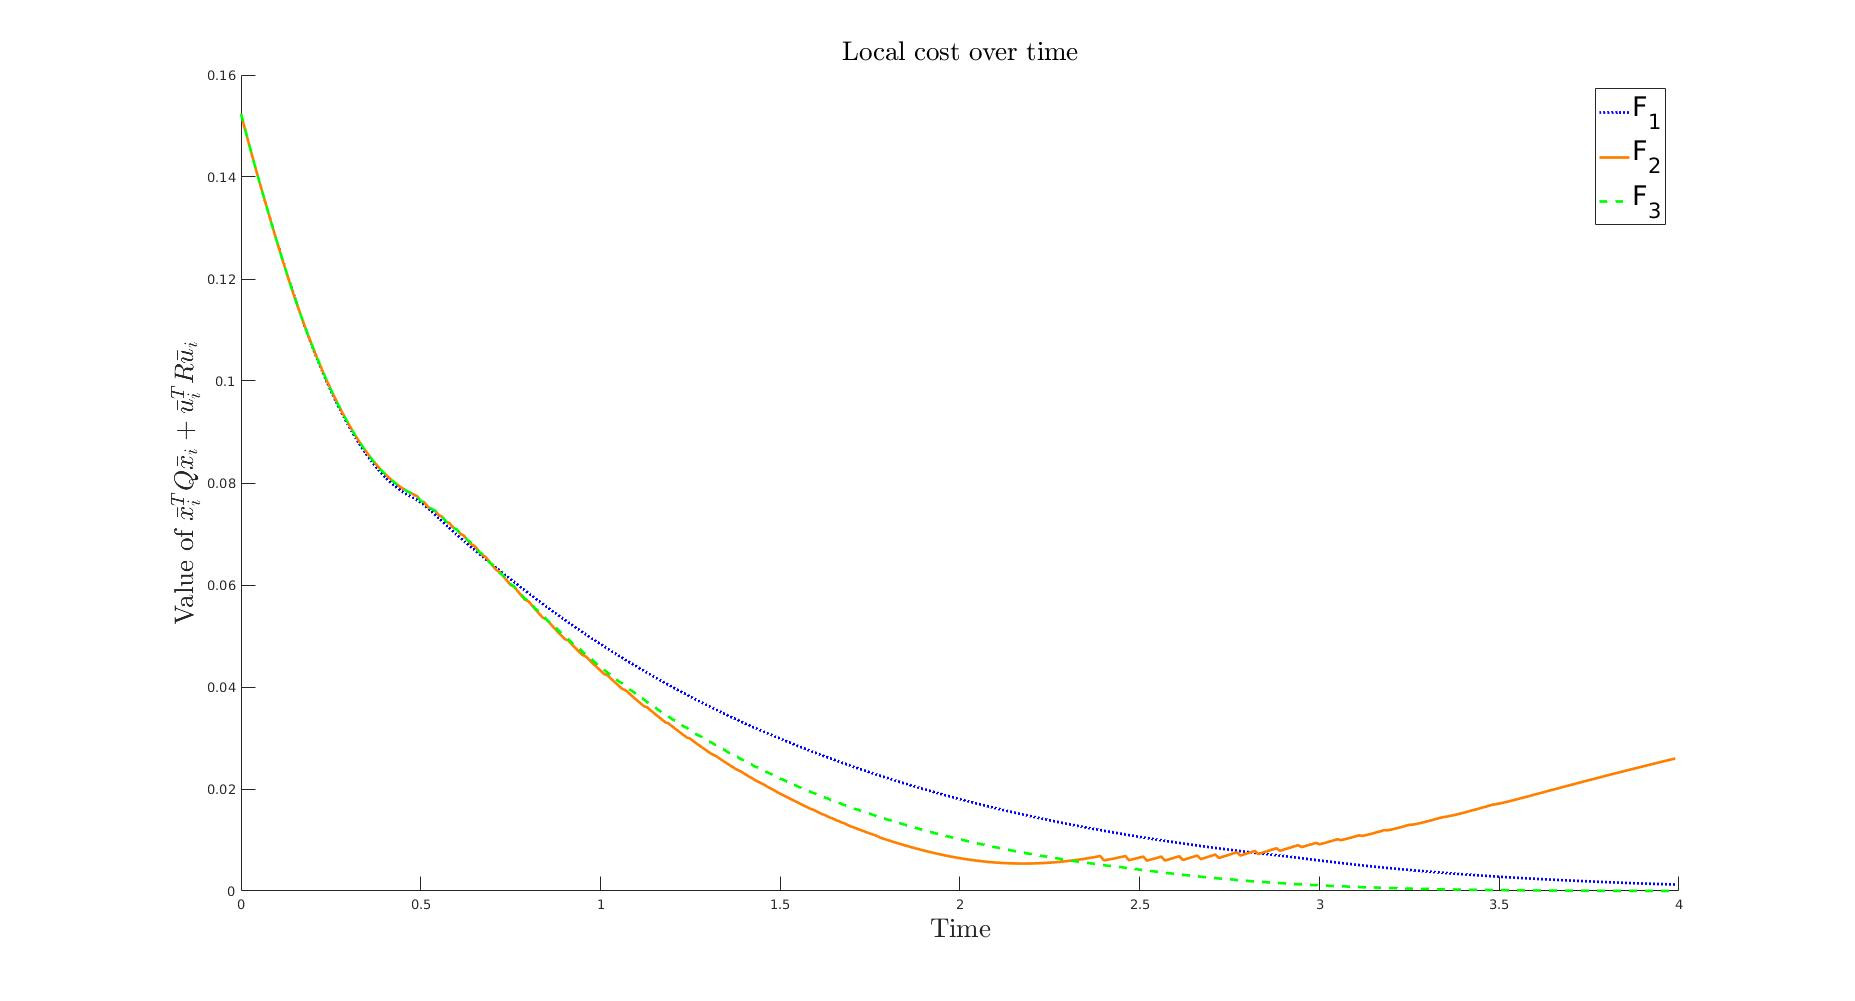
\includegraphics[width=16cm]{non_chameleon.jpg}
\end{center}
\caption{\label{fig:non_chameleon} \small Local cost over time for families $F_1$, $F_2$, and $F_3$ obtained following a straight line on the x axis and using an initial condition $\textbf{x}_0 = (0, 0.05, - \dfrac{\pi}{6}, 0)^T$.}
\end{figure}

The performance decrease experienced in $F_2$ can be explained by the fact that the FOM optimizer can choose optimal trajectories that will never be able to be applied. For example, the optimal control solution at a certain optimization iteration can be to choose the second mode of $F_2$: start with an L state for the first time step to then choose a R step and finally choose an S step for the rest of the finite time horizon prediction. The capability of sliding left and right should allow the pusher to take more aggressive turns by sliding to one of the slider edges and then slide back to the center to properly track the straight line. The main problem is that the control law for the controller is to execute the only th first step of the optimal trajectory, so the system will be in an L state for one time step and then the control law will be recomputed. As no mode starts with a sliding right state the slider can never go back to the central position.

The conclusion these experiences led us to was that, using Bersekas' terminology, some families did not have the sequential improvement property. What's more, the results seemed to indicate that composition or expansion of families that apparently had sequential improvement could lead to losing the property.

Solving the MPC using the FOM approach has similarities with the roll-out algorithm presented in their study: Each of the modes can be considered a heuristic and the strategy of recomputing the control policy at a certain frequency by using the same heuristics can be viewed as a roll-out-like technique. In fact, we could easily reformulate any family of our FOM approach to behave as their roll-out by increasing the finite horizon by one step and substitute each of the original modes by a triplet of copies preceded with an S, L, and R state respectively. We decided not to use an exact roll-out because, as we will show in this section, we were able to find a strategy to guarantee a sense of improvement without having to increase the number of MPC sub-problems to solve by a multiples of the number of possible states.

It's important to note that the concepts of sequential consistency or optimality cannot be applied to our case without some previous modifications, because of the existence of a receding finite time horizon, but for every FOM problem we can formulate an associated Full Horizon Family of Modes (FFOM) problem as follows: (TODO: Define it).

\begin{definition} {\textbf{FFOM:}}\\
Given a FOM problem defined by a finite horizon of $N$ steps, a set $H$ of possible hybrid states, a cost function J, and a family $F^{(0)} = \{M_1^{(0)}, ..., M_k^{(0)}\}$ containing k modes, where $M_i^{(0)}$ is a general mode described as $M_i^{(0)} = (s_{i,1}, s_{i,2}, ..., s_{i,N})$, with $s_{ij} \in H$. Furthermore, consider a cost function $J_k = \sum\limits_{i = k}^{N} \left( \diff{\textbf{x}}_i^T \textbf{Q} \diff{\textbf{x}}_i^{} + \diff{\textbf{u}}_{i}^T \textbf{R} \diff{\textbf{u}}_{i}^{} \right)$ (defined using the $\textbf{Q}$ and $\textbf{R}$ matrices from the FOM cost function J) and the prefixes of each of the modes of the family $M_i^{(j)} = (s_{i,1}, ..., s_{i,N-j})$. Then the associated FFOM problem is defined iteratively as follows:

\begin{enumerate}
\item Solve the FOM-based MPC problem defined by $F = F^{(0)}$ and $J = J_0$, using $x_0$ as the initial condition.
\item Use the controller $\diff{\textbf{u}}_0$ from the optimal solution of the problem solved in the previous step to compute the value of $\diff{\textbf{x}}_1$. Under an ideal world assumption (that is, assuming that our motion equations model is accurate) the value of $\diff{\textbf{x}}_1$ will correspond to the same value obtained in the optimal trajectory of the MPC.
\item Replace $F$ by  $F^{(1)} = \{M_1^{(1)}, ..., M_k^{(1)}\}$, $J$ by $J_1$, and the initial condition by $\diff{\textbf{x}}_1$ and go to step 1, solving this time an MPC problem of $N - 1$ steps.
\item Repeat until the horizon has only one step.
\end{enumerate}

\end{definition}


This formulation represents how the FOM problem would behave be if we had enough computation power to cover a finite horizon that reaches the desired final time step. Using it, we can study the FFOM problem associated to the example families presented at the beginning of this section. For simplicity, we will consider the realized states and control inputs to describe the considered trajectories.

\begin{example} \label{ex:f1consistent} $\textbf{F}_1$ \textbf{is sequentially consistent in it's FFOM version and assuming an ideal world:}

Consider that at a certain control iteration there's a full horizon of N steps to reach the end of the trajectory. The only considered mode, $\textbf{S}$, get the optimal path to reach the goal while keeping the sticking contact at all times, obtaining a sequence of position states $\textbf{x}^{\textbf{S}}(\textbf{x}_0) = (\textbf{x}_{1,1}, \textbf{x}_{1,2}, ..., \textbf{x}_{1,N})$ and control inputs $\textbf{u}^{\textbf{S}}(\textbf{x}_0) = (\textbf{u}_{0,1}, \textbf{u}_{1,1}, ... \textbf{u}_{1,N-1})$ for the optimal path from the initial position to the goal. Then, the controller will execute $\textbf{u}_0$ for one control step and the pusher slider system will move to $\textbf{x}_1$. The only heuristic it considers in the next optimization step is to stick until reaching the goal, so the optimal trajectory obtained will be $\textbf{x}^{\textbf{S}}(\textbf{x}_1) = (\textbf{x}_{1,2}, ..., \textbf{x}_{1,N})$ and $\textbf{u}^{\textbf{S}}(\textbf{x}_1) = (\textbf{u}_{1,1}, ... \textbf{u}_{1,N-1})$, being sequentially consistent.
\end{example}
\begin{example} \label{ex:f2notconsistent} \textbf{On the same conditions, $\textbf{F}_2$ is not sequentially consistent nor improving:}

Let's call the second mode of family $\textbf{LR}_1$. If this mode is chosen at a certain time step, giving an optimal trajectory $\textbf{x}^{\textbf{LR}_1}(\textbf{x}_0)$ and control $\textbf{u}^{\textbf{LR}_1}(\textbf{x}_0)$. In the next step, a mode $\textbf{R}_1$ is required in the family to consider the continuation of the previous optimal trajectory, which consists in sliding right and then sticking until the end of the trajectory. As it is not the case, the new FFOM step will not consider the previously optimal trajectory and, if no relation can be proven between the trajectories considered in the current step and the ones considered in the previous step, neither consistency nor improvement cannot be guaranteed.
\end{example}


Consider that, at a given step of a FFOM problem, the initial position is given by $\textbf{x}_0$ and the optimal trajectory is determined by the mode $M_1^{(0)} = (s_{1,1}, s_{1,2}, ..., s_{1,N})$. If the family contains a mode whose maximal prefix corresponds to the maximal suffix of $M_1^{(0)}$, $M_2^{(0)} = (s_{1,2}, ..., s_{1,N}, s_{2,N+1} )$ then sequential improvement will be guaranteed at the next iteration step. That is, if the trajectory provided by $M_1$ at the first step is $\textbf{x}^{M_1^{(0)}}(\textbf{x}_0) = (\textbf{x}_1, \textbf{x}_2, ..., \textbf{x}_N)$ and $\textbf{u}^{M_1^{(0)}}(\textbf{x}_0) = (\textbf{u}_0, \textbf{u}_1, ..., \textbf{u}_{N-1})$ and the one provided by $M_2$ at the second step is $\textbf{x}^{M_2^{(1)}}(\textbf{x}_1) = (\textbf{x'}_2, ..., \textbf{x'}_N)$ and $\textbf{u}^{M_2^{(1)}}(\textbf{x}_1) = (\textbf{u'}_1, ..., \textbf{u'}_{N-1})$, then

\begin{lemma} \label{lem:seq_imp} {$J_1(\textbf{x}^{M_2^{(1)}}(\textbf{x}_1),\textbf{u}^{M_2^{(1)}}(\textbf{x}_1)) = J_1(\textbf{x}^{M_1^{(1)}}(\textbf{x}_1),\textbf{u}^{M_1^{(1)}}(\textbf{x}_1))$:}


As $M_2^{(1)}$ is the maximal suffix of $M_1^{(0)}$ the continuation of the trajectory provided by $M_1$ on the first step is feasible in the mode $M_2$ during the second step so, as the trajectory given by $M_2$ is optimal, $J_1(\textbf{x}^{M_2^{(1)}}(\textbf{x}_1),\textbf{u}^{M_2^{(1)}}(\textbf{x}_1)) \leq J_1(\textbf{x}^{M_1^{(1)}}(\textbf{x}_1),\textbf{u}^{M_1^{(1)}}(\textbf{x}_1))$

If we assume $J_1(\textbf{x}^{M_2^{(1)}}(\textbf{x}_1),\textbf{u}^{M_2^{(1)}}(\textbf{x}_1)) < J_1(\textbf{x}^{M_1^{(1)}}(\textbf{x}_1),\textbf{u}^{M_1^{(1)}}(\textbf{x}_1))$ we can easily reach a contradiction. Let's define $\textbf{x}^* = (\textbf{x}_1, \textbf{x'}_2, ..., \textbf{x'}_N)$ and $\textbf{u}^* = (\textbf{u}_0, \textbf{u'}_1, ..., \textbf{u'}_{N-1} )$. This is a feasible trajectory in $M_1^{(0)}$ but $J_0(\textbf{x}^*, \textbf{u}^*)$ can be expressed as: $$J_0(\textbf{x}^*, \textbf{u}^*) = \textbf{x}_0^T \textbf{Q} \textbf{x}_0 + \textbf{u}_0^T \textbf{R} \textbf{u}_0 + J_1(\textbf{x}^{M_2^{(1)}}(\textbf{x}_1),\textbf{u}^{M_2^{(1)}}(\textbf{x}_1))$$ and we can conclude that $J_0(\textbf{x}^*, \textbf{u}^*) < \textbf{x}_0^T \textbf{Q} \textbf{x}_0 + \textbf{u}_0^T \textbf{R} \textbf{u}_0 + J_1(\textbf{x}^{M_1^{(1)}}(\textbf{x}_1),\textbf{u}^{M_1^{(1)}}(\textbf{x}_1)) = J_0(\textbf{x}^{M_1^{(0)}}(\textbf{x}_0),\textbf{u}^{M_1^{(0)}}(\textbf{x}_0))$, reaching a contradiction.
\end{lemma}

Let's now consider an extension state E. That is, a default state to apply mode extensions. We can then define a mode suffix operation as follows.

\begin{definition} {\textbf{Mode Suffix Operation:}}

Given a default extension state E, applying the suffix operation to mode $M_1 = (s_1, s_2, ..., s_N)$ results in $M_2 = suff(M_1) = (s_2, ..., s_N, E)$
\end{definition}

This definition allows us to announce the following corollary from lemma \ref{lem:seq_imp}.

\begin{corollary} \label{cor:seq_imp} {A family $F$ closed by a suffix operation is sequentially improving in the FFOM problem:}

At any step $i$ of the approximated MPC, a certain mode $M$ will provide the optimal trajectory. As $suff(M) \in F$ we can use lemma \ref{lem:seq_imp} to guarantee that the trajectory provided by $suff(M)$ in step $i + 1$is as good as the one currently provided by $M$. As the approximated MPC considers the optimal trajectory between all the considered modes, the computed trajectory at $i + 1$ will be at least as good as the one computed in $i$.
\end{corollary}

\begin{example} \textbf{On the same conditions, $\boldsymbol{F_3}$ is sequentially improving:}

$F_3$ is closed by the suffix operation defined using $S$ as the extension state, so we can use corollary \ref{cor:seq_imp} to guarantee sequential improvement in the FFOM.
\end{example}

We considered important to guarantee sequential improvement for the FFOM problem even taking into account that our problem is not in the ideal world (modelling errors and different frequencies for the optimization problem and the controller can lead the state obtained when applying $u_0$ to $\diff{x_0}$ to be different from $x_1$) and that we don't have a full horizon. As we showed in the examples above, the simulation results were in agreement with these theoretic results as the families that implicitly guaranteed sequential improvement in their FFOM version tended to outperform the ones that did not.

In order to guarantee it we decided first decided to only use families that were closed by the suffix operation obtained using $\textbf{S}$ as the extension mode. The problem with this approach is that for any mode $M = (s_1, ..., s_N)$ you add to a family F you need to include all of its possible $\textbf{S}$-extended suffixes. Different modes required adding a different number of suffix modes. For example, an $\textbf{S}$ mode required no extra modes (as it is itself closed by the suffix operation) and for a $\textbf{R}_n$ one you only need to extend the family with an $\textbf{S}$ mode and all the $\textbf{R}_i$ modes for $i < n$. Even taking this into account, we considered adopting this strategy constrained the problem of family design more than we wanted to and added more extra nodes that was strictly necessary, so we decided to adopt another strategy. This translated into changing from static families to dynamical ones.

(TODO: Explain why $\textbf{S}$)

The strategy we used consisted in including a dynamic mode that we called chameleon mode. If, at a certain step $i$, the optimal FOM mode is mode $M$, the chameleon mode is defined in step $i + 1$ as $suff(M)$ (using, as before, $\textbf{S}$ as the extension state). This guaranteed sequential improvement by applying lemma \ref{lem:seq_imp} in an analogue way as in corollary \ref{cor:seq_imp}.

The chameleon mode functionality was added in the simulation interface and it's performance was tested in simulation. As we will show in section \ref{subsec:simresults}, implementing this functionality resulted in an improvement of the sequential behaviour of the FOM algorithm. Being able to safely add arbitrary new modes to the FOM family without fear of losing its sequential properties allowed us to develop an strategy to learn a good family set-up for a general trajectory tracking problem, as will be shown in chapter \ref{sec:modeselection}.

Given the good properties of the chameleon mode, we decided to include it in the FOM formulation so, from now on,we will use FOM to refer to the family of modes with chameleon mode implementation, unless specified otherwise.

\subsection{MIQP and Clustered MIQP}
\label{subsec:miqp}

We wanted to compare the solutions provided by FOM with traditional MPC solving techniques. In order to do that we decided to implement the MIQP technique using the commercial solver Gurobi. This solver was already used in Hogan's work in a force-based formulation prior to the final velocity-based one. This formulation was not presented in the final paper, but it allowed to formulate an MIQP problem that was able to run in an average of 3Hz. It should be mentioned that the execution time at every control iteration could range between few milliseconds to 10 seconds depending on the initial condition of the MPC.
This is not a problem for simulation, but in a real control environment the frequency at which you can update the controller is not bounded by the average frequency at which you can solve the MPC, but by the worst case scenario one. Otherwise the controller may try to update the control input before it is computed by the optimizer. There may be solutions to this effect in other formulations, but for the one used in Hogan's work the MIQP controller could run at more than 0.1Hz.

We were expecting a similar behaviour in the velocity-based formulation, but it took several orders of magnitude more time to solve each iteration. In order to simulate 500 simulation steps with a finite horizon of 7 steps it took an average of 6 hours of execution time, which implies that the maximum control frequency we could apply would probably not surpass 0.02Hz, a clearly insufficient frequency. We were expecting to have an "ideal" MIQP result to compare FOM with and try to get similar results with FOM with less computational effort, but the results obtained with 7 steps of the MIQP were worse than the FOM and we couldn't afford to increase the horizon further.

We looked at techniques to speed up the MIQP execution in the Gurobi website and we found out that our current big-M formulation worked better (both in execution time and in quality of the obtained trajectory) than the indicator constraints formulations as smaller the M parameter was. As explained in \ref{subsec:mpc_formulation} each M parameter used in a scalar inequality $Ax \leq b + M (1 - z)$ must be greater than $\max\limits_{x \in D}{(Ax - b)}$ (where D is the domain of possible values of the x) so that the inequality is rendered redundant when z = 0. We implemented a version of MIQP that given a vectorial constraint as the ones used in Hogan's formulation $A\vec{x} \leq \vec{b} + M (1 - z) \cdot (1, ..., 1)^T$ replaces the arbitrary constant M by a vector $\vec{M}$ where each component's value is $M_i = \max\limits_{x_i \in D}{(A_i x_i - b_i)}$. We were not able to improve the execution time, but we were able to obtain better results for the MIQP. The results showed in the next section for the MIQP will use this optimized big-M formulation.

In order to compare FOM to other methods using a longer time horizon, we implemented another MPC solving method based on MIQP that we called Clustered MIQP. Given a standard MPC formulation, this method works in the following way:

\begin{itemize}
\item Consider a clustering factor $c$, a finite horizon $ N \cdot c$ and a set of h hybrid states $ \{ H_1, ..., H_h \}$.
\item The finite horizon is then divided into N clusters of c steps: $(C_1, ..., C_N)$.
\item The state space is extended with 3 binary variables per step $(s_i, d_i, u_i)$ for a total of 3N variables.
\item Each variable $s_i$ $d_i$ and $u_i$ is associated with the hybrid state of the cluster $C_i$ (sticking, sliding down and sliding up respectively).
\item The constraint $s_i + d_i + u_i = 1$ is enforced 
\item The problem constraints are formulated with big M notation or indicator constraints and the problem is fed into an MIQP solver.
\end{itemize}

This way we can reduce the dimensionality of the optimization problem by keeping the same state during all the steps of the same cluster. The execution time of this new problem is similar to the execution time of a MIQP problem of N steps but the controller inputs can be different at each of the $N c$ steps.

We intended to use this method to approximate MIQP problems with long horizons (around 35 steps) by using few clusters (around 5) and we expected to obtain a better trajectory than the ones obtained with FOM. As will be discussed later, the results of this MIQP approximation were worse than the results obtained in FOM with a good choice of few modes.

\subsection{Simulation Conclusions (TODO)}
\label{subsec:simresults}

We tested our chameleon mode implementation by comparing the performance of families of modes that are not sequentially consistent in their full horizon formulation with and without the chameleon mode with satisfactory results. In Figure \ref{fig:chameleon} we show the example presented in section \ref{subsec:chameleon}. All the simulation parameters are kept the same except for the usage or non usage of the chameleon mode. As can be observed, the results correspond with our expectations: for the family $F_2$ the chameleon mode implementation successfully tracks the trajectory while the implementation without it failed to do it, as we showed previously.

\begin{figure}[htb!]
\begin{center}
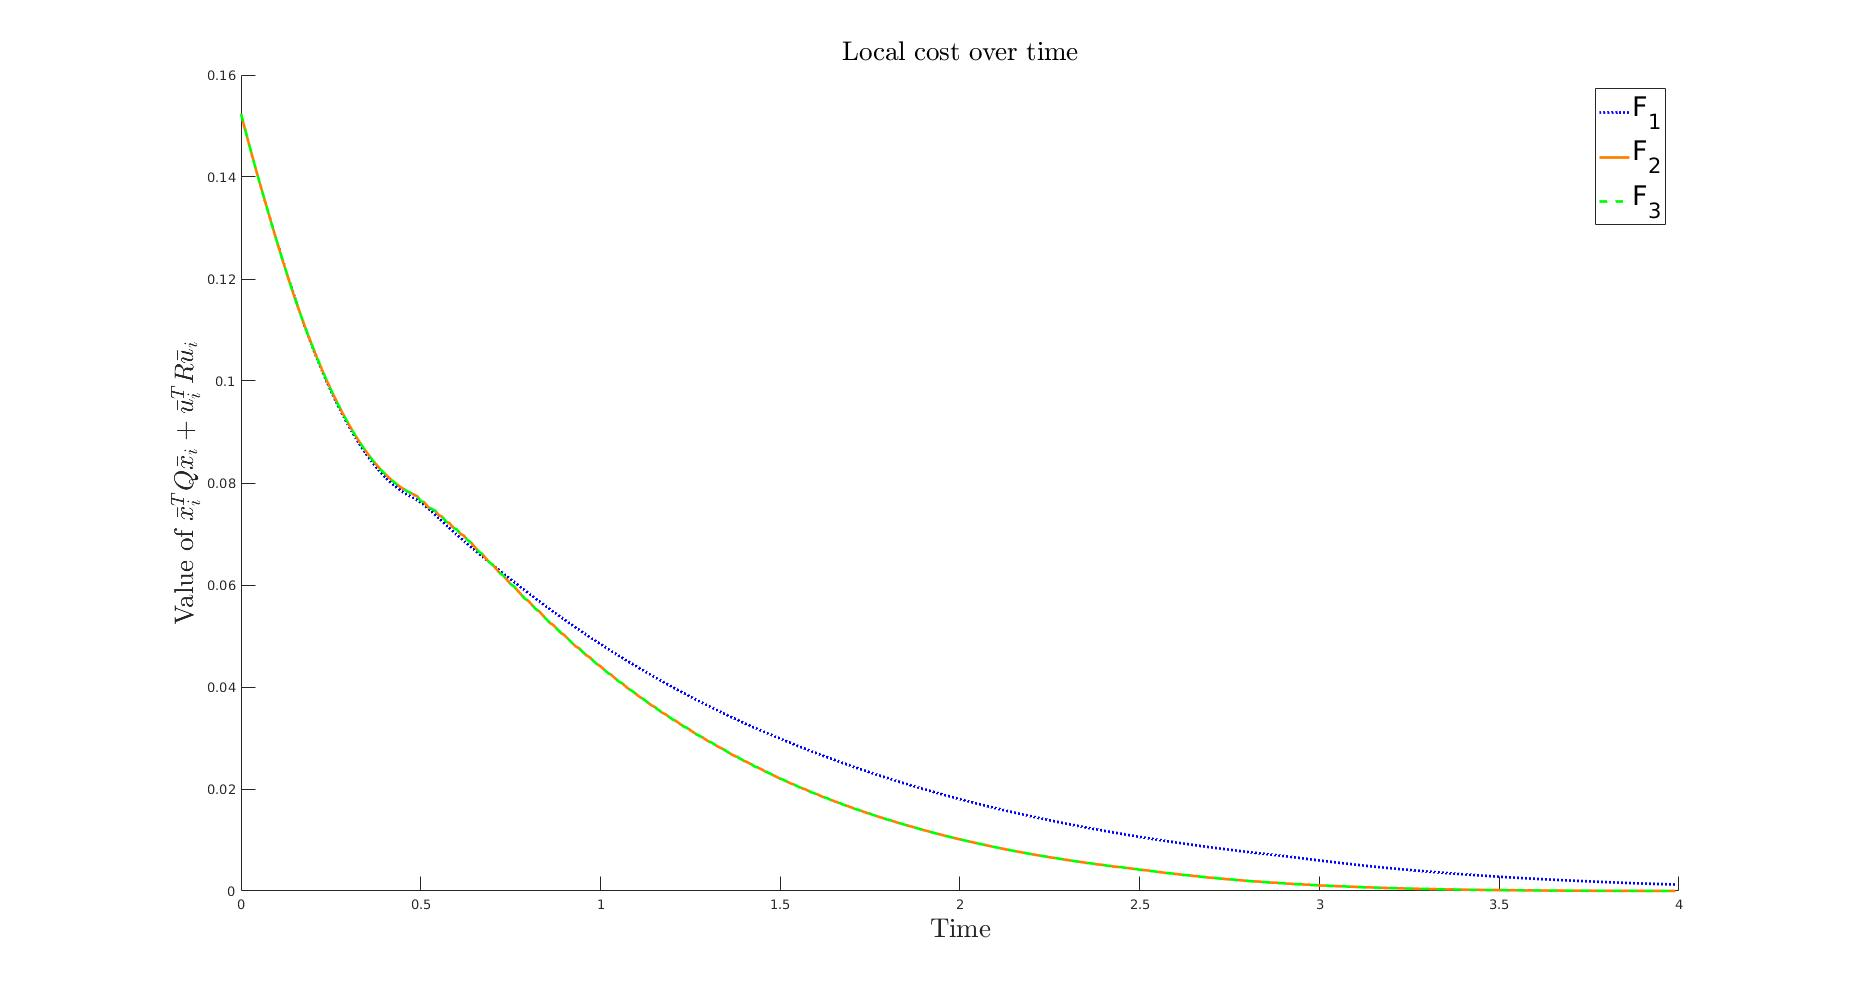
\includegraphics[width=16cm]{chameleon.jpg}
\end{center}
\caption{\label{fig:chameleon} \small Local cost over time for families $F_1$, $F_2$, and $F_3$ obtained following a straight line on the x axis and using an initial condition $\textbf{x}_0 = (0, 0.05, - \dfrac{\pi}{6}, 0)^T$.}
\end{figure}

We were able to compare both MIQP and FOM with a small finite horizon of 5 steps and we were able to observe the expected behaviour: Some families gave poor results when compared to MIQP, but the result could be iteratively improved by adding new modes. The obtained trajectories did not strictly follow an increasing sequence, but 

Finally, we compared clustered MIQP with five clusters of 7 steps with a FOM approach using three modes family formed by the S, $U_1$, and $D_1$ modes. 

\section{Mode Selection Protocol}
\label{sec:modeselection}
In the previous sections it is explained how we addressed the sequential properties of the FOM formulation and provided a metric and other MPC solvers to compare FOM to. At this point of our study, we were able to adress our next objective: To optimize the selection of the family modes for the FOM formulation.

We considered multiple optimization criteria and relations to study and we had to adopt a set of assumptions to be able to obtain some initial results. For our first study, we tried to learn the modes to follow a single fixed straight line trajectory. Each optimization problem would be parametrized by a fixed finite time horizon (characterized by a number of steps N) and a fixed number of modes K a family could contain. The initial condition $\diff{x_0}$ was assumed to be a random variable following a certain probability distribution. The cost of the control trajectory C was thus also a random variable of unknown distribution parametrized by the optimization problem parameters. Specifically given a set of K modes $\{m_1, ..., m_k\}$, $C \sim D(m_1, ..., m_k)$ for a given distribution law D. Ideally, we would like to choose the the set of modes that minimizes $\mean{C}$.

We made three main assumptions:
\begin{assumption} \label{ass:localcost}
\textbf{Local Cost Sufficiency:} Optimizing the modes to reduce the local costs obtained while solving each MPC iteration would be sufficient to obtain a low global cost.
\end{assumption}
\begin{assumption} \label{ass:localinv}
\textbf{Locally Invariant Trajectories (TODO: Check it's a good name:)} Given a local inertial frame F centered on the slider center of mass moving and rotating with it and given an infinite objective trajectory $C(t)$ for $t \in (-\infty, \infty)$, then the $C(t)$ would be time invariant in frame F (for example an infinite circle loop or an infinite straight line).
\end{assumption}
\begin{assumption} \label{ass:singlestep}
\textbf{Single Step Sufficiency:} A single control iteration of the trajectory tracking problem was sufficient to learn which modes where optimal, if the appropriate distribution for $\diff{x_0}$ was chosen.
\end{assumption} 

The motivation and justification for these assumptions will be explained in \ref{subsec:structure}, as well as some other implicit assumptions contained in it. In \ref{sec:todo} we will discuss some of the studies we would have conducted and how we would have modified these assumptions if we disposed of more time.

\subsection{Structure Study And Systematic Approach}
\label{subsec:structure}
Given a finite horizon of N steps and H states and considering M the set of possible modes obtained by concatenating N of these hybrid states, then $|M| = H^N$. Let the set of possible families containing K of these modes be F. Then $|F| = \binom {|M|}{K} = \frac{H^{N}!}{K!(H^N-K)!}$. Even with a low number of states this number grows quickly as N and K increase.

If we tried to directly tackle the optimization problem without any assumption or knowledge of its structure, we would need to solve several trajectory tracking problems for each of these possible families, because the families could be correlated between themselves. A simple example that will probably clarify this effect is that a $D_1$ or $U_1$ family will probably perform poorly alone because if the pusher slides away from the center of the slider face it will never be able to go back to it and control near the edges of the face is less versatile than on the middle (for example, while steeper turns can be taken in the edges of the face, changing rotation direction is much more difficult, at some point not even possible without sliding to the other side).

Solving many different initial conditions for all possible mode combinations with a long enough finite horizon would take too much time even to learn the optimal modes to track a single trajectory. We didn't want to use any simplification that would be specific to our pusher-slider system, because we wanted to provide systematic tools to use the FOM approach in general problems the control community may face. This led us to use a set of general assumptions to simplify the problem and devise a systematic protocol to study the structure of each problem and use different optimization/learning techniques depending on the structure.

We mentioned the local cost sufficiency assumption again here, but this assumption was already taken when deciding to use a finite horizon MPC formulation to control the pusher-slider system. The mode selection will determine the performance of our local FOM solver and the relation between local MPC performance and overall performance and the validity of this assumption were already discussed in \ref{subsec:costfunc} and \ref{subsec:simresults}.

The locally invariant trajectories assumption motivation will be explained later in \ref{subsec:dynfom} (TODO: Make sure I don't forget to explain it)

The main motivation for the single step sufficiency assumption has to be understood under the previous assumption. The locally invariant property implies that the only difference between an MPC step and another is their initial condition random variable $\diff{x_i}$. Consider a distribution law X that focusses more on covering a wide range of possible values of any $\diff{x_i}$ rather than on their frequency as, for example an appropriate uniform distribution. We can then optimize the modes to reduce the expected value of $C(\diff{x_0})$ of a single controlling step tracking problem, where $\diff{x_0} \sim X$. Optimizing the mode selection this will simultaneously reduce the local costs expected value for all $\diff{x_i}$ implicitly assuming that each of these values are equally distributed.

This implicit assumption is clearly false. The fact that some trajectories converge is already a counterexample of it. We consider assuming a uniform to describe all $\diff{x_i}$ is a conservative approach, as will consider rare big disturbances (that can usually only happen with an external perturbation or a bad initial position) to be equally likely to appear at any time step as small disturbances characteristic of proper control around the objective trajectory. We expected this approach would be sufficient to provide a mode selections that would be robust enough to track a wide range of trajectories and initial conditions, but that could fail to capture some feedback relations between modes. This will be further discussed in \ref{sec:todo}.

These assumptions result in a great cost reduction and simplification of the learning algorithm because the optimization problem can be now be easily written as a function of $\diff{x_0}$:
\begin{corollary} \textbf{The optimization problem to select the FOM modes can be expressed as:} \label{cor:costfunction} 
 $$\min\limits_{m_1, ..., m_K \in M}\mathbb{E}(C(\diff{x_0}; m_1, ..., m_K)) = \min\limits_{m_1, ..., m_K \in M}\mathbb{E}(\min\limits_{i = 0}^{K}{C_i(\diff{x_0})})$$
 
\end{corollary}
Where $C_i$ is the cost associated to mode $m_i$ in the MPC optimization. This further implies that solving the MPC problem for all the possible sets of K modes is no longer necessary. If $C_i(\diff{x_0})$ is computed for every mode $m_i \in M$, then $C(\diff{x_0}; m_1, ..., m_K)$ is defined for any set of K modes by corollary \ref{cor:costfunction}.

This algorithmic cost reduction was not enough to face the full learning problem. We no longer had to study the full space of families F, but we still had no alternative to explore the full space of modes M, even if we just try to obtain a local minimum. Many local optimization techniques can avoid considering the full space it by relying on the structure of the optimization problem. For example, when the parameters are on a continuous metric space, the concept of gradient arises and methods as gradient descent can be used. Some structures can also be used to guarantee stronger properties as in convex problems, were local solutions are also global.

Considering all these aspects, we devised a systematic approach to study the structure of a general MPC problem and optimization techniques. We then provided a set of optimization techniques to be applied to obtain an approximate solution for the optimization problem. It has to be noted that the studies and techniques we will present are not proofs of a certain structure and thus, the techniques do not guarantee any kind of optimal solution. We considered proving any of these properties in an specific problem to be an object of research study in itself and it escaped the goal of this thesis, as we wanted to provide general simple tools to expand the FOM usage in the manipulation community.

TODO: Maybe get rid of all this last part, never been a fan of it.
\begin{itemize}
\item {Finite horizon increase sensibility:}
\item {Mode metric study:} In section (TODO:reference it) we provide and discuss a mode metric. We wanted to study if there was a continuity-like property (if we bound the bound distance between modes we can bound to some extend the distance of their costs). Having this property would allow to 
\item {Cost distribution study:} If all have the same distribution, fewer samples would be required, or at least we could have boundaries on the error.
\end{itemize}

\subsection{Simulation Results. Simple trajectory learning}
\label{subsec:learningsimple}
For our initial study, we tried to learn the best modes for single locally invariant trajectories. As proposed in the previous section, we started by obtaining 1000 samples of $\diff{x}$ from a uniform distribution in a cube in $\mathbb{R}^4$ the $\diff{x}$ and $\diff{y}$ disturbances on the x and y position of the slider center of mass were bounded between 0.5 and 0.5 meters. The slider angle disturbance $\diff{\theta}$ was bound between -$\dfrac{\pi}{4}$ and $\dfrac{\pi}{4}$ and the value of $p_y$ could lay in any point on the slider surface. For each initial condition the tracking problem was solved for all the possible modes with a small finite horizon of 5 steps. This implied 243 possible modes to be solved for each of the 1000 initial conditions, for a total of 243.000 single step tracking problems. The cost functions $C_i(\diff{x_j})$ were computed for each mode-initial condition pair. In Figure \ref{fig:hist_pre} 

\begin{figure}[htb!]
\begin{center}
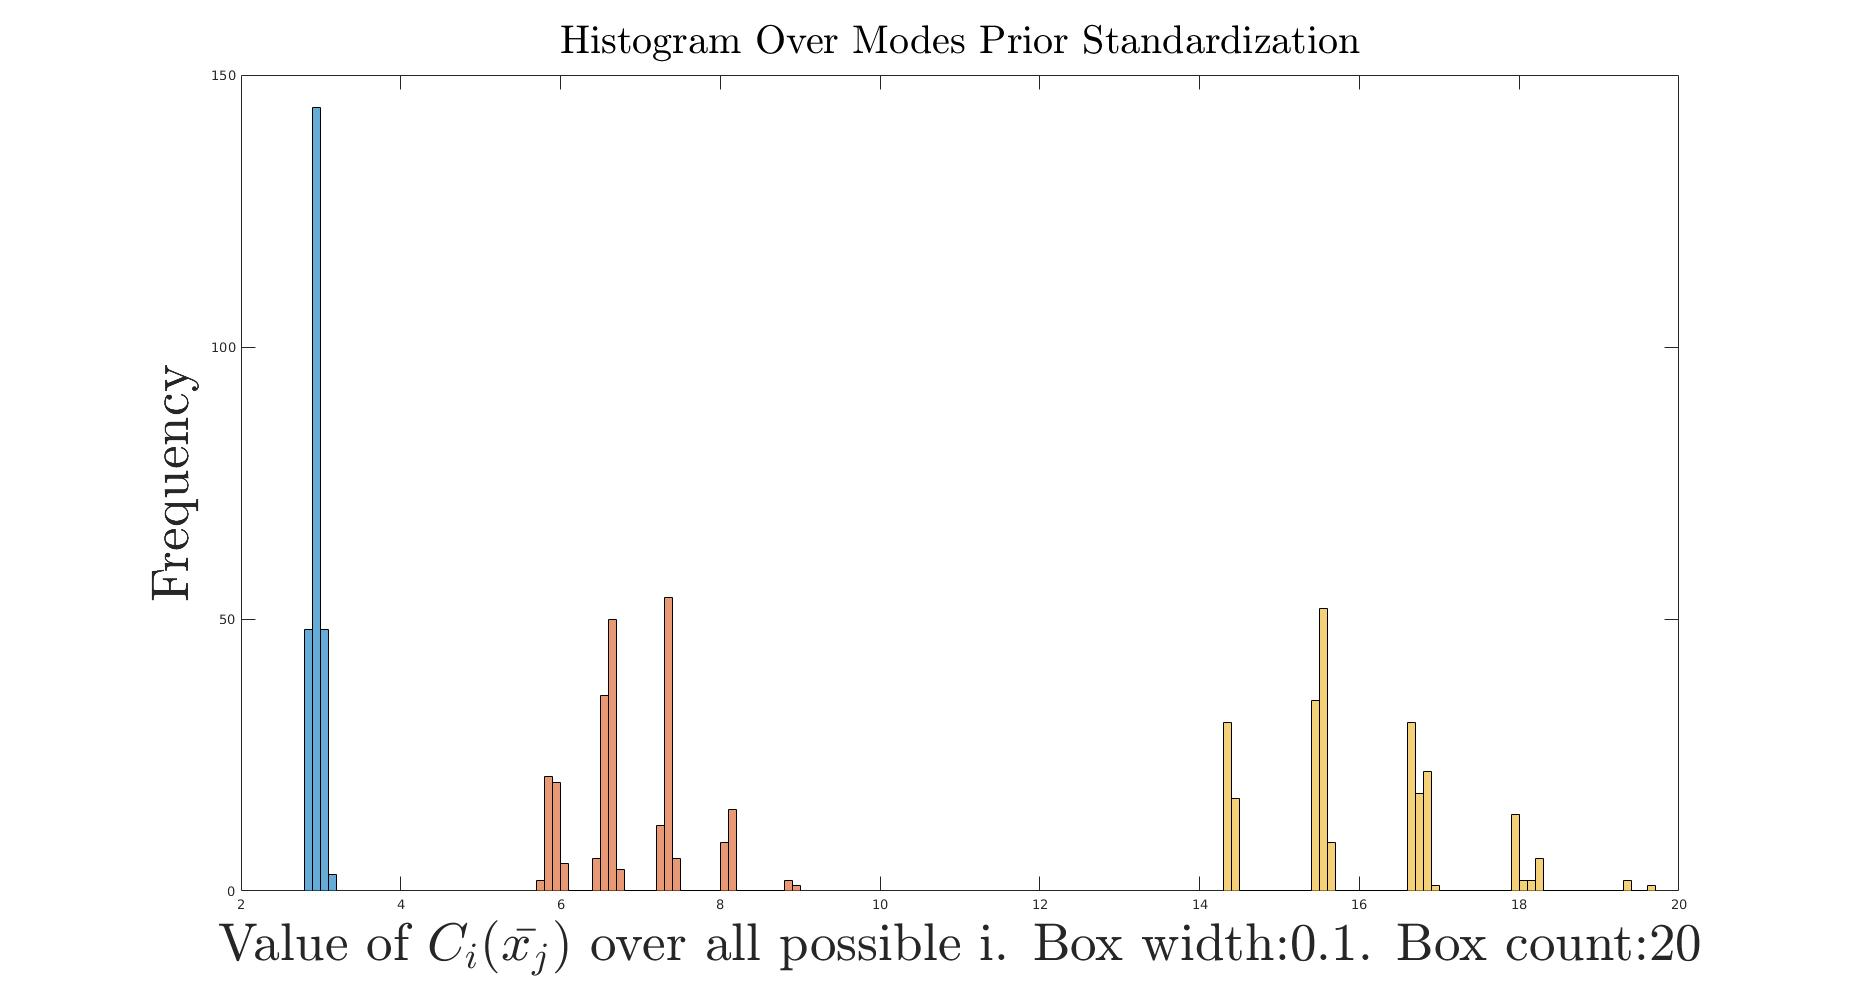
\includegraphics[width=16cm]{hist_pre_std.jpg}
\end{center}
\caption{\label{fig:hist_pre} \small Example histogram of $C_i(\diff{x_j})$ of the local costs obtained while tracking a horizontal line for 1000 initial conditions. The costs are clearly non-comparable}
\end{figure}

% trajectory described by $\textbf{x}(t) = (0.05 t, 0, 0, 0)^T$, $\textbf{u}(t) = (0.05, 0)$ with a finite horizon of 5 steps. The initial conditions were of the form $\textbf{x}_0 = (0, -0.5 + (i-1) \cdot 0.001, 0, 0)^T$, and a line as objective trajectory.

\begin{figure}[htb!]
\begin{center}
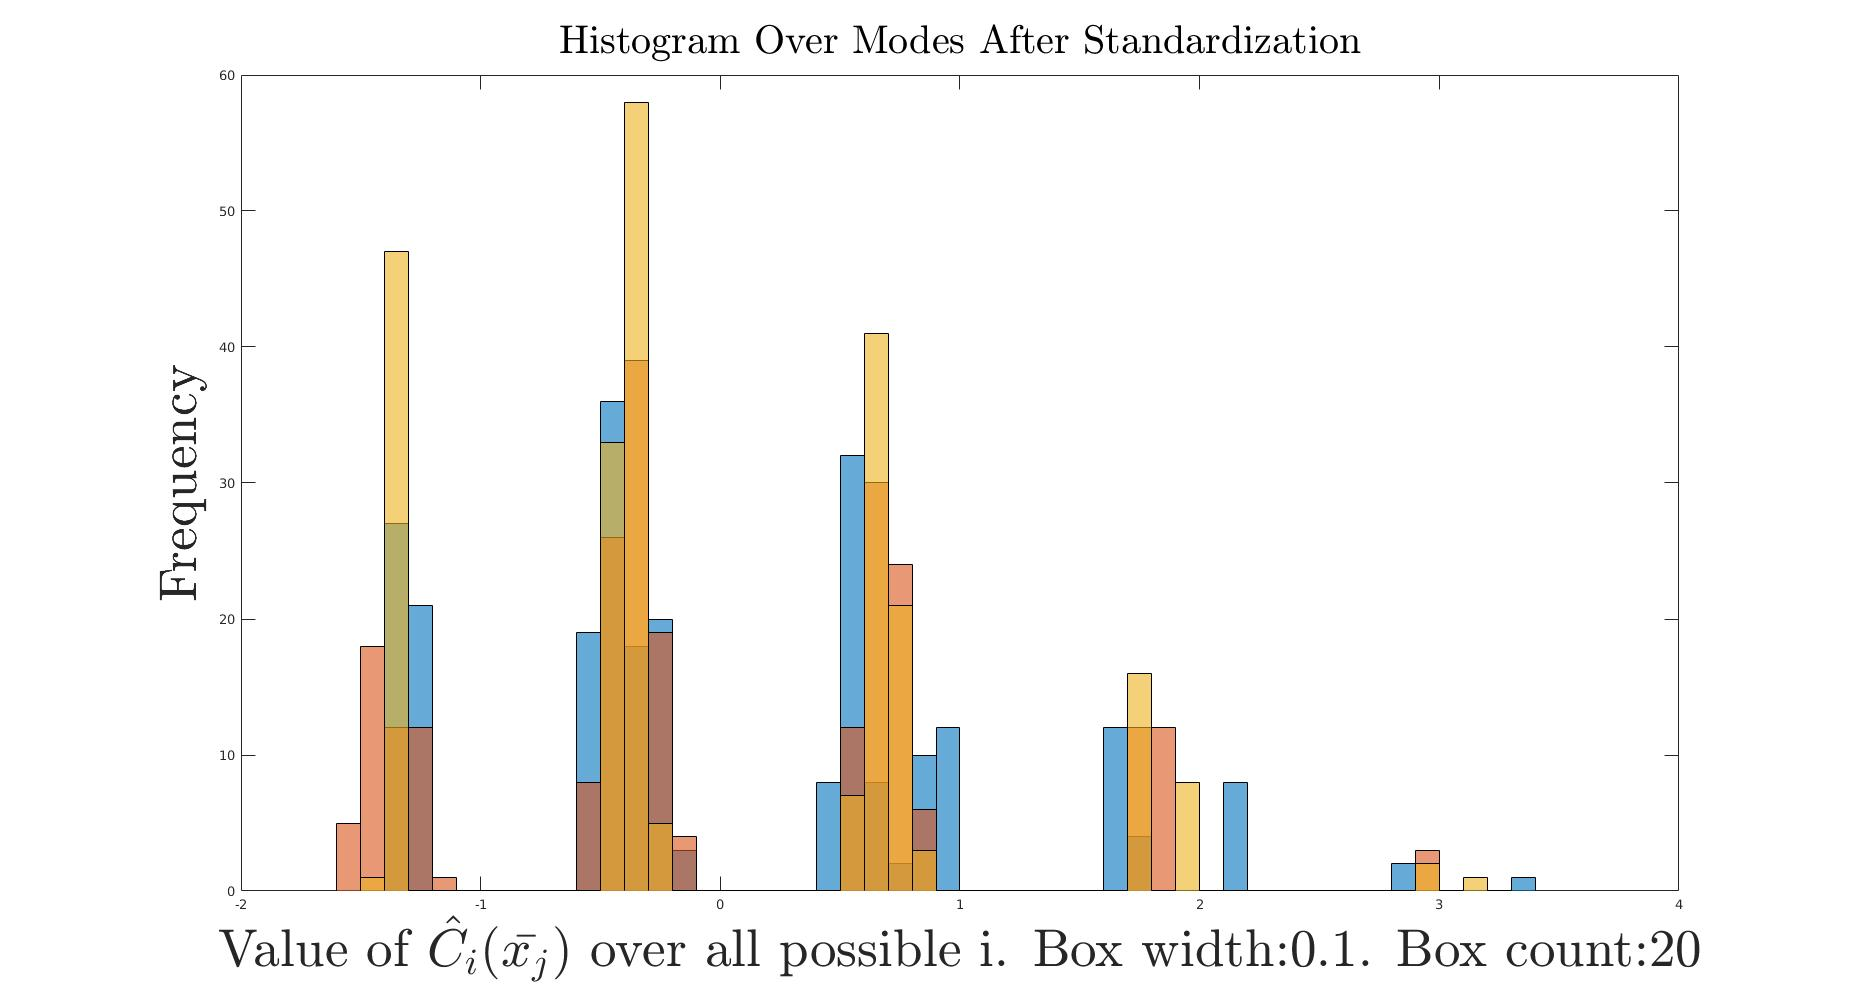
\includegraphics[width=16cm]{hist_after_std.jpg}
\caption{\label{fig:hist_post} \small Example histogram of $\hat{C_i}(\diff{x_j})$ for the same simulation set-up as in Figure \ref{fig:hist_pre}. The costs are now comparable}
\end{center}
\end{figure}

We were concerned that the initial condition had a lot of effect in the overall cost of the mode-condition pair, because higher or smaller disturbances would lead to higher or smaller overall cost respectively, independently of the mode chosen, and the simulation results confirmed it, as can be seen in Figure \ref{fig:hist_pre}. We wanted to reduce the impact of the initial condition in the range of possible values of the local costs to  obtain comparable experiments, so we decided to standardize the results obtained within each experiment. That is, given $C_i(\diff{x_j})$ we computed $\mean{C_i} = \dfrac{\sum\limits_{j = 0}^{243}{C_i(\diff{x_j})}}{243}$ and $\sigma_i = \sqrt{\sum\limits_{j=0}^{243}{\dfrac{(C_i(\diff{x_j}) - \diff{C_i})^2} {242}}}$ and we used them to compute $\hat{C_i}(\diff{x_j}) = \dfrac{C_i(\diff{x_j} - \diff{C_i})}{\sigma_i}$. The resulting standardized costs can be observed in Figure \ref{fig:hist_post}.

We were not able to determine a clear probabilistic distribution for $\hat{C_i}(\diff{x_j})$ so we decided to minimize the statistical mean for each distribution $ \bar{C}(\diff{x}; m_1, ..., m_K) = \frac{\sum\limits_{j=0}^{N}{\min\limits_{i = 0}^{K}{C_i(\diff{x_j})}}}{N}$.

Choosing the set of K modes that minimizes the desired expression can depend exponentially on K, so we used a greedy upper bound approximation to compute it. The greedy approach was defined recursively as follows:
\begin{lemma}\textbf{Upper bound to } $ \bar{C}(\diff{x}; m_1, ..., m_K)$\textbf{:}
(TODO: Define)
\end{lemma}
A dynamic programming algorithm was then implemented to simulate the recursion. Furthermore, we determined the lower bound of $ \bar{C}(\diff{x}; m_1, ..., m_K)$ by computing the minimum over all the modes for each experiment and computing the statistical mean.  $\min\limits_{m_1, ..., m_K \in M}\mathbb{E}(\min\limits_{i = 0}^{K}{\hat{C_i}(\diff{x})})$. By comparing the evolution of our computed upper bound with the lower bound we can see that the approximate algorithm quickly converges to the optimal solution (see Figure \ref{fig:cost_over_modes}) this properly captures relations between modes. The algorithm can choose modes that, even if they would not provide small means by themselves, can greatly increase their performance by associating with modes that specialize in initial conditions where they fail to give a good result. (TODO: Explain Better. For example say that the min mean for one is -1.6 and that it get's closer)

\begin{figure}[htb!]
\begin{center}
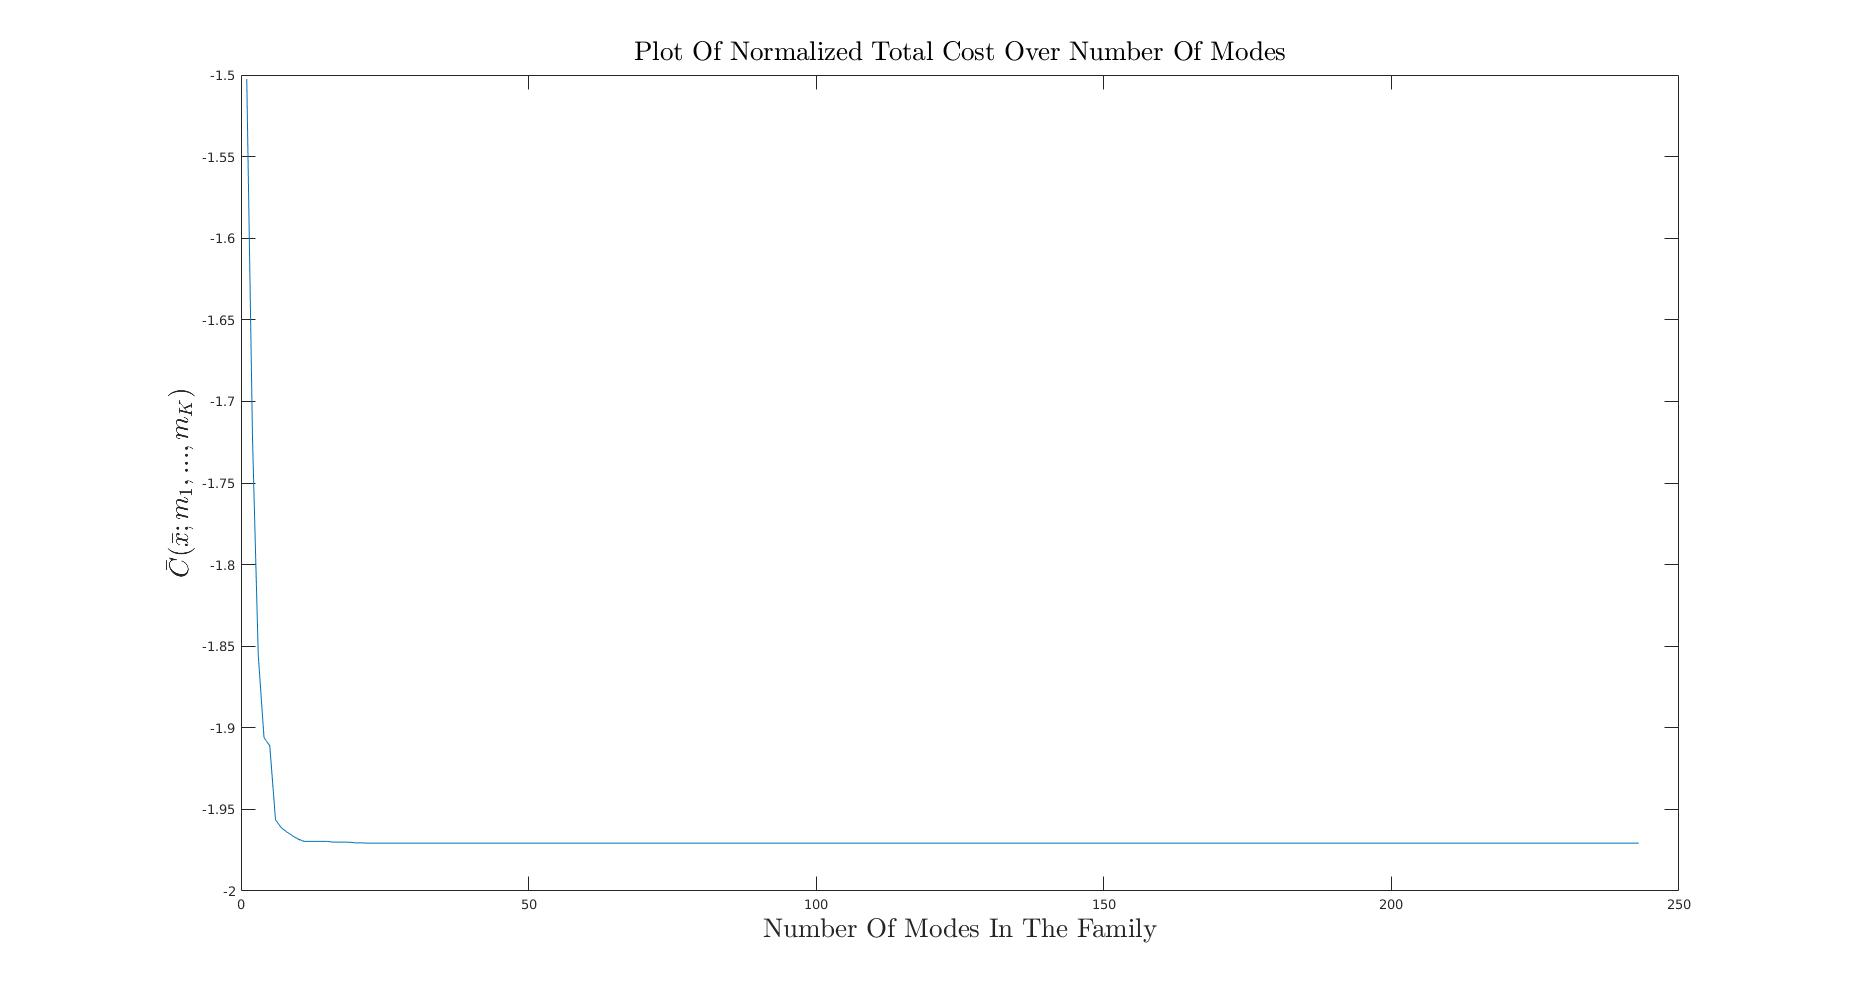
\includegraphics[width=16cm]{cost_over_modes.jpg}
\caption{\label{fig:cost_over_modes} \small Plot of our greedy approximation to the minimum value of $\diff{C}(\diff{\textbf{x}}; m_1, ... m_K)$ obtained by using families with K modes. The horizontal bar shows the optimal lower bound obtained when all the families are used. It's exact value is -1.9633.}
\end{center}
\end{figure}

We then proceeded to follow the strategies cited in the previous section. We successfully computed an approximation of the best modes for a 35 step length horizon by iteratively selecting the 5 best modes for $5 \cdot i$ steps for $i \in [1, 6]$ and extending them to $5 \cdot (i + 1)$ steps by adding all the possible tails to the previous best modes. Experimental results showed that state differences were more important when they occurred near the beginning of the mode than the end. This motivated us to compare the results obtained by following the full iterative procedure and the results obtained by computing the best modes for a short horizon and extending it with a long simple tail.

(TODO: add pictures of the comparisons)

\begin{figure}[htb!]
\begin{center}
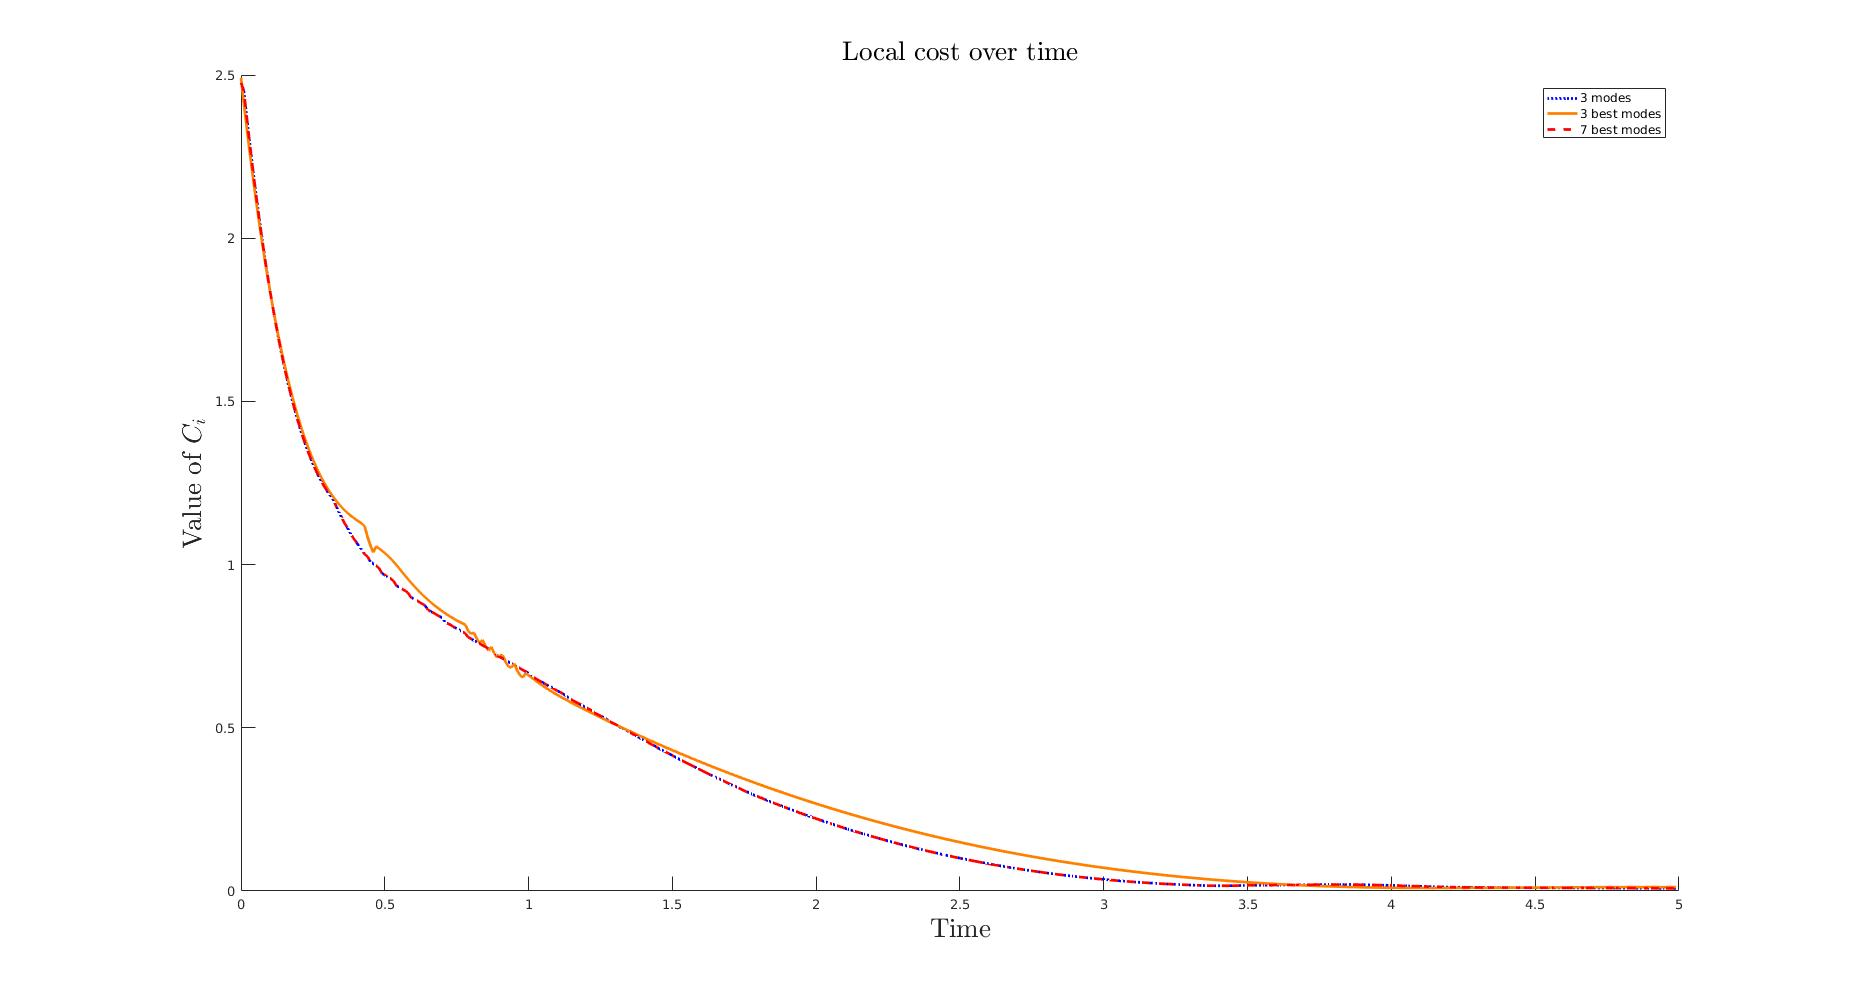
\includegraphics[width=16cm]{learning_straight.jpg}
\caption{\label{fig:cost_over_time_line} \small Comparison between the original FOM from Hogan's study and the families obtained by the learning algorithm. The initial condition is $\diff{\textbf{x}}_0 = (0, .05, \dfrac{\pi}{6}, 0)^T$. The vertical axis correspond to the optimal value of the finite horizon MPC over time.}
\end{center}
\end{figure}

\begin{figure}
    \centering
    \begin{minipage}{0.45\textwidth}
        \centering
        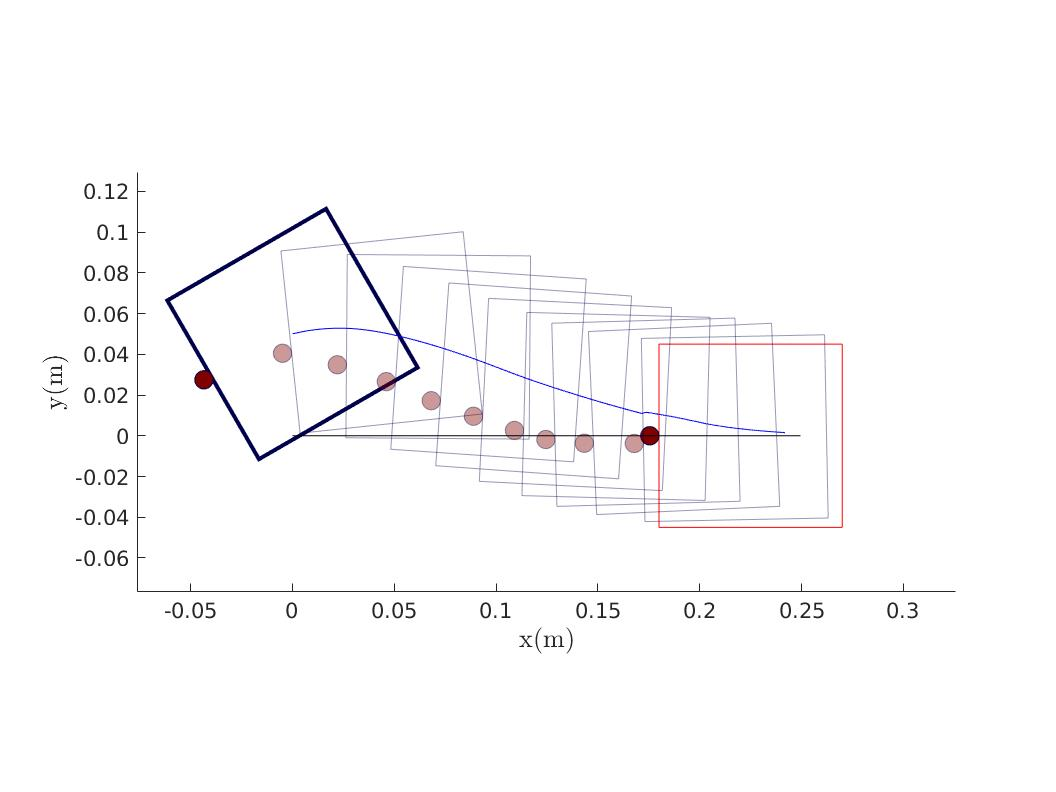
\includegraphics[width=1\textwidth]{learning_straight_original.jpg} % first figure itself
        \caption{Trajectory obtained with the family from Hogan's work. Overall cost: 11.8847}
    \end{minipage}\hfill
    \begin{minipage}{0.5\textwidth}
        \centering
        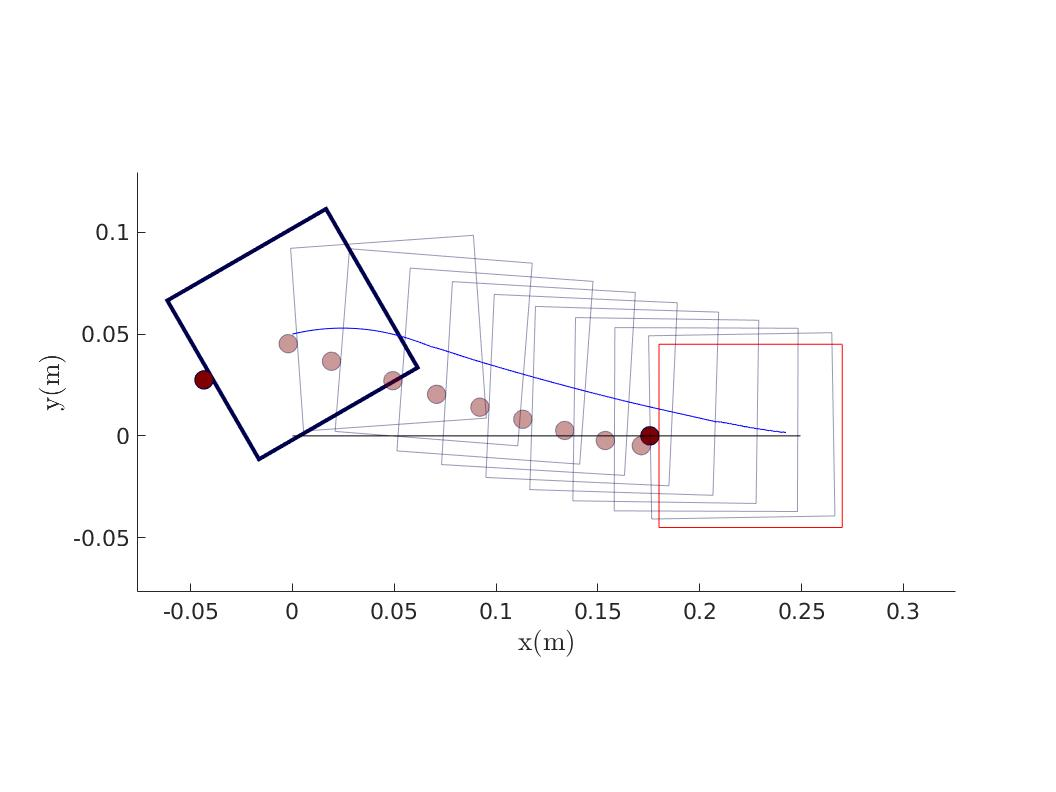
\includegraphics[width=1\textwidth]{learning_straight_3_modes.jpg} % second figure itself
        \caption{Trajectory obtained with the best combination of three modes computed using our learning procedure. Overall cost: 11.8664}
    \end{minipage}
\end{figure}

The results obtained showed that adding a simple sticking tail to the best K modes chosen for a short trajectory was enough to successfully track a trajectory. (TODO: study with different tail)

(TODO: add graph with this)

Experimental results also showed that the improvement obtained by adding new modes decreased exponentially (TODO: check the proper name for this) before reaching the optimal value, as can be seen in Figure \ref{cost_over_modes}. After a few modes, the results are highly stable and the changes in the cost function are small.

Finally, we tested the robustness of the method by tracking circular trajectories with the best modes obtained for a straight line. The behaviour was completely different if the initial condition was outside or inside of the tracking circle. As can be seen in (TODO) few modes were sufficient to properly track trajectories with high external disturbances. On the other hand, small internal disturbances could lead to solutions with a steady state error that ended tracking a circle internal to the one determined by the objective trajectory if few modes were used. Progressively adding modes steadily reduced the effect.

\begin{figure}[htb!]
\begin{center}
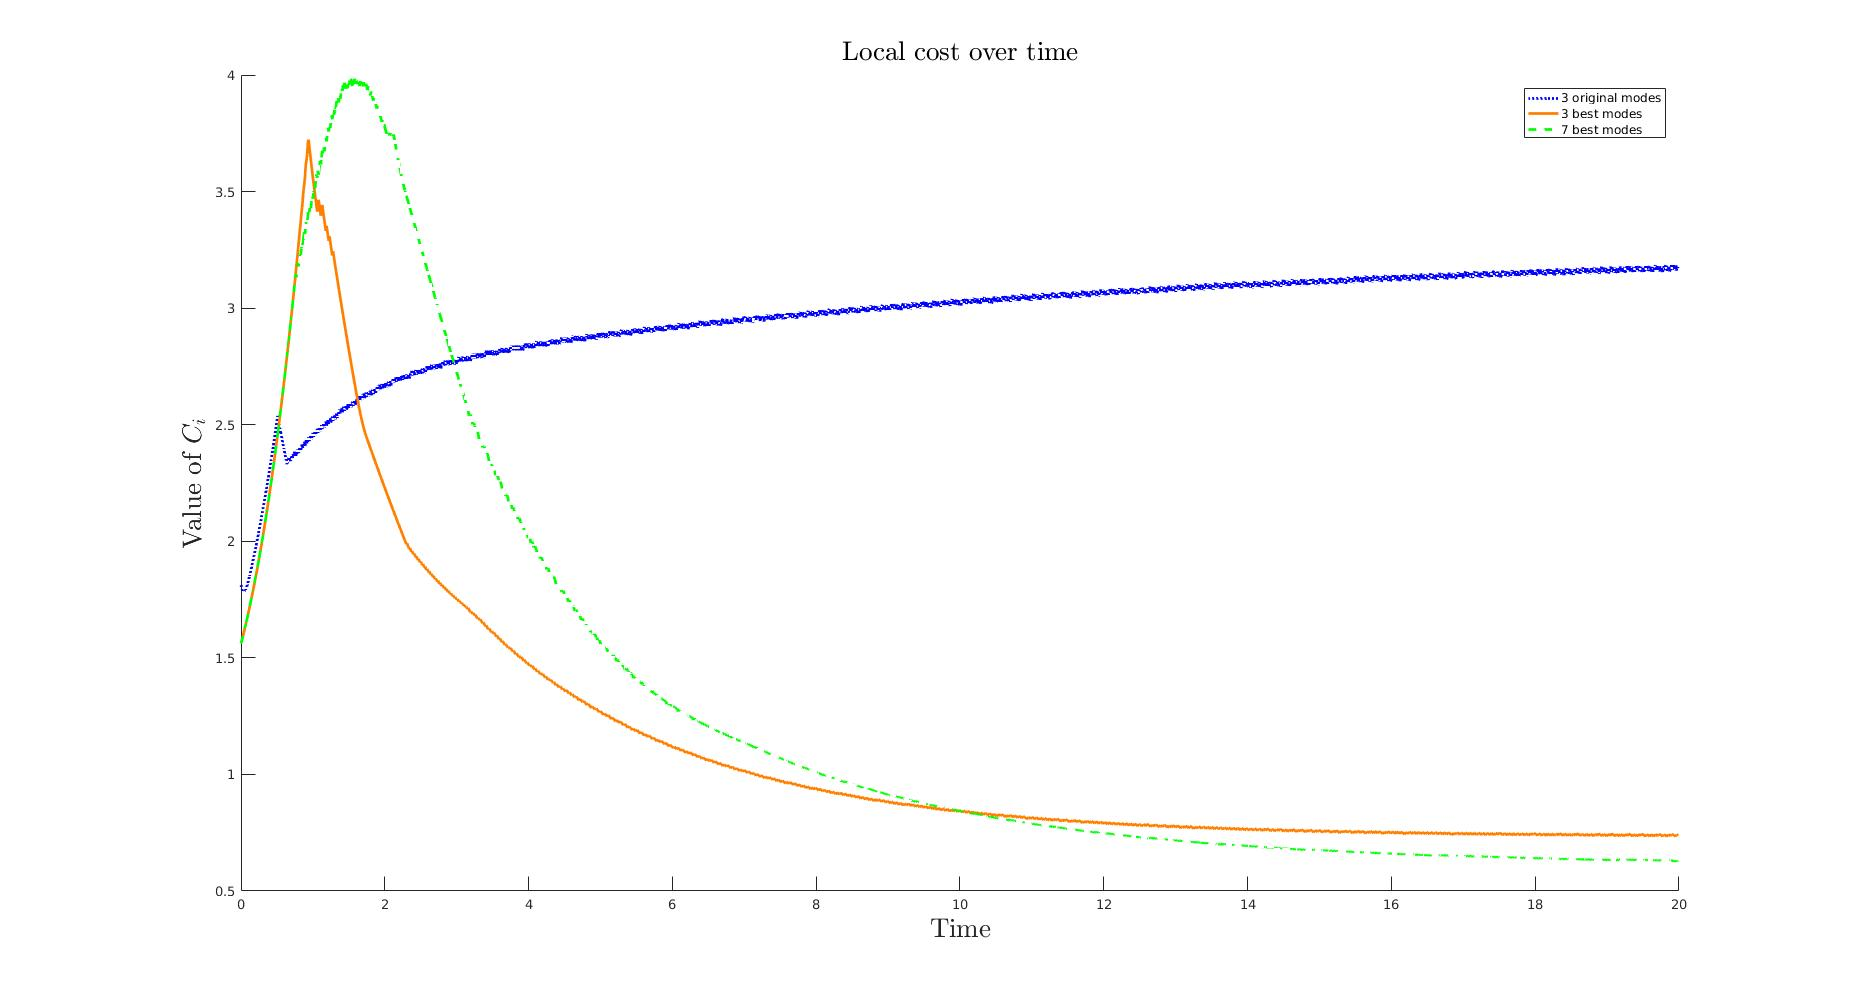
\includegraphics[width=16cm]{old_vs_new_circle_interior.jpg}
\caption{\label{fig:old_vs_new_circle_internal} \small Analogue to Figure \ref{fig:cost_over_time_line} for a circle trajectory with a internal disturbance. The initial condition is $\diff{\textbf{x}}_0 = (0.0, -0.03, -0.1, 0.0249)^T$}
\end{center}
\end{figure}

\begin{figure}
    \centering
    \begin{minipage}{0.5\textwidth}
        \centering
        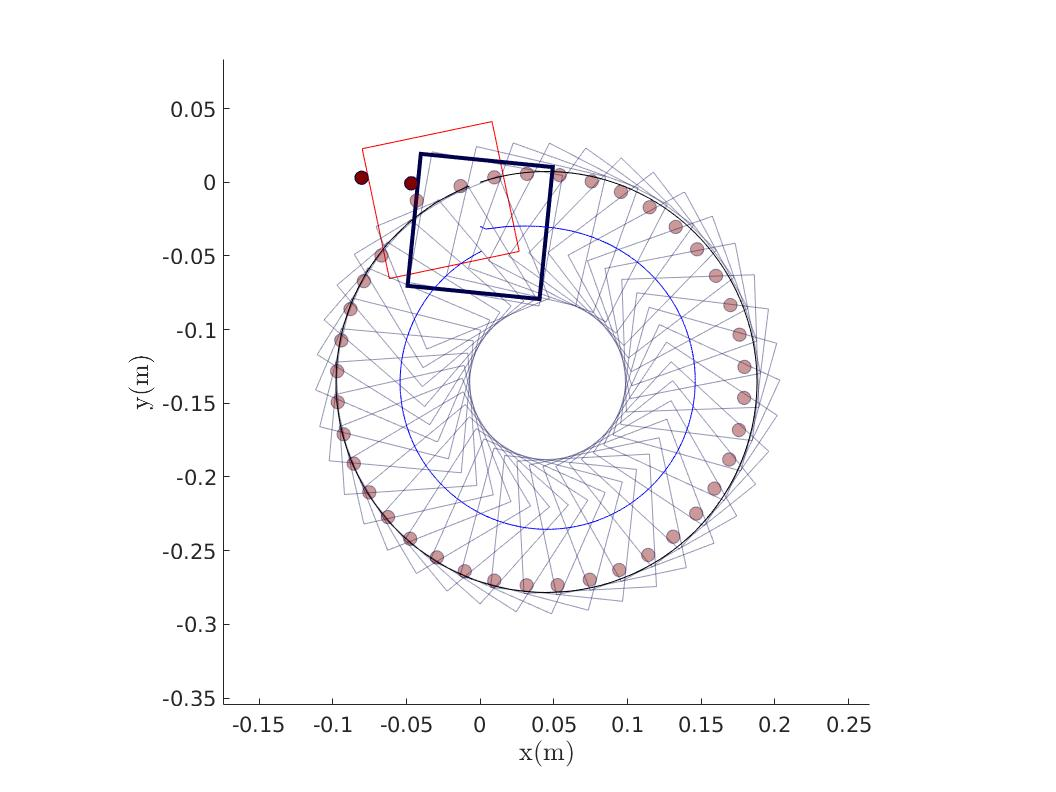
\includegraphics[width=1\textwidth]{frank_modes_circle_internal.jpg} % first figure itself
        \caption{Trajectory obtained with the family from Hogan's work. Overall cost: 195.2719}
    \end{minipage}\hfill
    \begin{minipage}{0.5\textwidth}
        \centering
        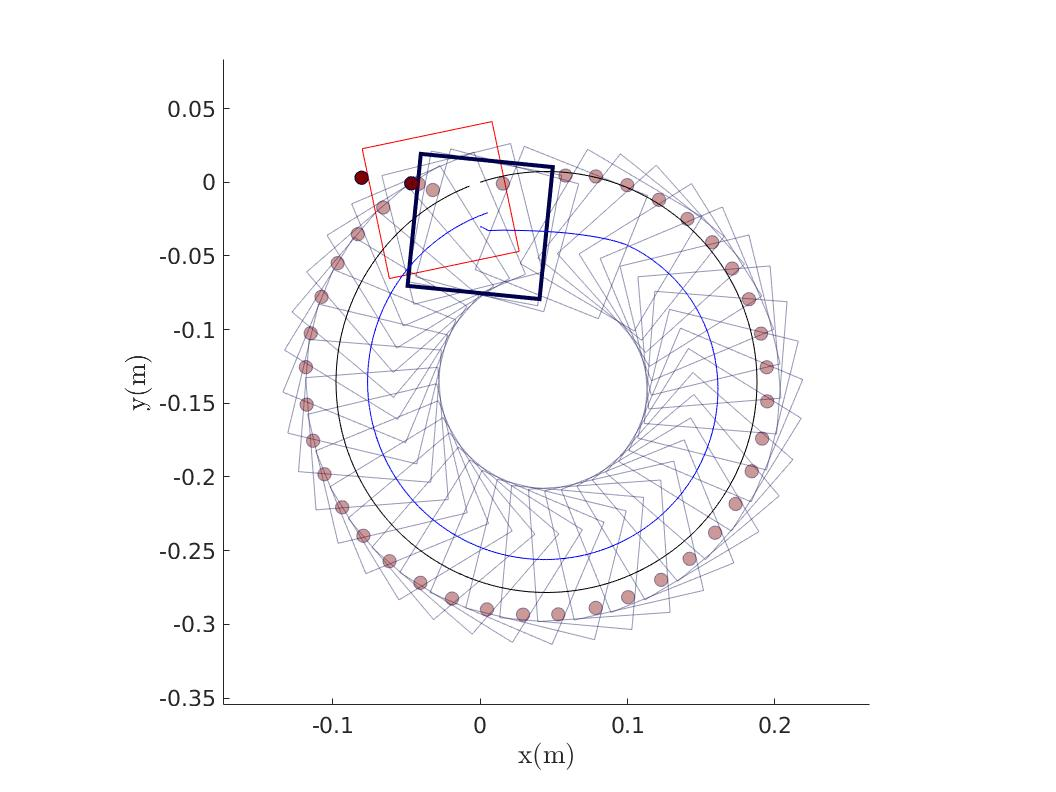
\includegraphics[width=1\textwidth]{best_3_modes_circle_interior.jpg} % second figure itself
        \caption{Trajectory obtained with the best combination of three modes computed using our learning procedure. Overall cost: 79.2438}
    \end{minipage}
\end{figure}

TODO: Circle with circle modes

\subsection{Dynamic FOM}
\label{subsec:dynfom}
The assumption of local invariance for the objective trajectories limited the range of application of the FOM approach as presented until now. In the previous section we could show a certain degree of robustness when using the modes learned on a simple straight line to track other trajectories, but the number of modes per family had to be increased while tracking circular trajectories in order to achieve the same results than while tracking straight lines.

As we mentioned in section \ref{subsec:structure}, we already had a motivation to use locally invariant trajectories before obtaining the simulation results from the previous section. Our goal was to train the FOM method on several base locally invariant trajectories that could describe most of the situations the tracking problem would face (For the simple contact pusher-slider system this consisted in a straight line and several circular trajectories of different curvatures). Then we wanted to learn the best k modes for every base trajectory. To track complex trajectories, we would approximate them as a piece-wise composition of base ones and at each controller step we would use the best modes for each base trajectory depending on the base trajectory approximation of the current step.

\begin{remark}
We will use the common mathematical notation for the curvature sign. That is, a positive curvature means that the unit tangent vector rotates counter-clockwise as a function of the parameter along the curve.
\end{remark}

The simulation results from  the previous section showed that the initial part of the modes generally held more importance than the last part. This motivated us to simplify the approximation of the general trajectory with a simple local approximation. We expected that a sufficient control frequency would allow the system to properly track the general trajectory even if its local properties undertook steep temporal changes. For the pusher-slider system mentioned before, the base trajectory was chosen by numerically computing the curvature of the objective trajectory at every control step and using the base trajectory with the most similar curvature value.

The chameleon mode brought the idea of having dynamic modes in a family and, in a similar way, the dynamic FOM brought the concept of having dynamic families in an MPC problem. At each control step, the best base trajectory to describe the local geometry of the objective trajectory was chosen. Then, the best k modes for that base trajectory were used (together with the chameleon mode) to solve the MPC problem on that instant. The chameleon mode was shared between the dynamical families to ensure that the sequential consistency property was not lost.

The main motivation for this method was to reduce the online cost of the FOM approach at the expense of more offline computations. We expected that choosing the best family dynamically would reduce the number of modes per family required to obtain good results in a broad range of trajectories. Having n modes in a family implies solving n convex optimization problems at every control step. The cost of solving each optimization problem may vary, so we cannot directly assume that the overall execution time of the algorithm is proportional to the number of modes in the family, but experimental results show so for our specific problem (TODO: add graph). Even without these experimental results, we still consider important for the control problems to reduce the online computational cost of the algorithm.

In the next section we will present the simulation results obtained while tracking a complex trajectory by using the dynamic FOM and a static FOM learned to track a straight line.

\section{Experiments}
\label{sec:experiments}

\section{Conclusion and Discussion}
\label{sec:conclusion}
\begin{enumerate}
\item{MIQP} takes too long, it's execution time depends on the geometry of the problem (different time at each iteration). The results may depend on the implementation chosen. If you don't have a software that allows you to tune everything it is too complicated to implement. Clustered MIQP is no better. We should try MIQP with tail (we expect good results but bad time)
\end{enumerate}

\section{Things to do if we had time}
\label{sec:todo}
\begin{itemize}
\item Study modes correlation
\item Study optimal mode dependency wrt initial condition.
\item Change the uniformly distributed initial conditions by normally distributed.
\end{itemize}

\section{Adding the MAMME cover page to your document}
\label{sec:coverPage}
  
Regardless of the structure of the document of your TFG, you have to use the template \texttt{coverTFG-GM.doc} for the cover page. You can follow the fowolling steps:
\begin{itemize}
	\item Generate a pdf file with the document of your TFG, following or not this template
	\item Modify the document \texttt{coverTFG-GM.doc} with the data of your thesis and generate a pdf with two pages (cover and blank page)
	\item Use Adobe or other sofware to join (combine or merge) the two pdf files in one pdf file. 
\end{itemize}
 
\newpage

\bibliography{fom_bib}{}
\bibliographystyle{plain}

%______________________________________________________________
\appendix
\vfill\newpage \section{Simulation Interface Code}
\label{app:code}
You can include here an appendix with details that can not be included in the core of the document. You should reference the sections in this appendix in the core document.

\end{document}


